\documentclass[11pt, spanish]{article}
\usepackage[spanish]{babel}
\selectlanguage{spanish}
\usepackage[utf8]{inputenc}
\usepackage{amsmath}
\usepackage{amsfonts}
\usepackage{amsthm}
\usepackage{float}
\usepackage{graphicx}
\usepackage{subcaption}

% Margenes
\usepackage[left=2cm,right=2cm,top=2cm,bottom=2cm]{geometry}
%Espaciado
%\linespread{1.3}


\title{Introducción al Procesamiento Digital de Imágenes - Práctica 6}
\date{}
\author{Gonzalo Ciruelos Rodríguez (LU: 63/14)}

\begin{document}
\maketitle

Para preparar el entorno para poder ejecutar todos los programas,
primero debe tenerse instalado \texttt{python3} (y su \texttt{pip} correspondiente).
Luego, debe ejecutarse 
\begin{verbatim}
    virtualenv -p python3 venv 
    . venv/bin/activate
    pip install -r requirements.txt 
\end{verbatim}

\noindent para instalar las dependencias (pillow (para imágenes), numpy y matplotlib).



\section{Ejercicio 1: Generación de casos de test para los ejercicios que siguen}

Modo de uso
\begin{verbatim}
    python3 practica6/ej1.py <img> <outputdir>
\end{verbatim}

Se utilizaron las imágenes \texttt{lena.png} y \texttt{test.png}, alterandolas con ruido gaussiano con media 10, ruido
gaussiano con media 50, ruido rayleigh con parámetro 1.5 y ruido salt \& pepper con probabilidad 0.1.

A continuación se encuentran las imágenes.

\begin{figure}[H]
\centering
  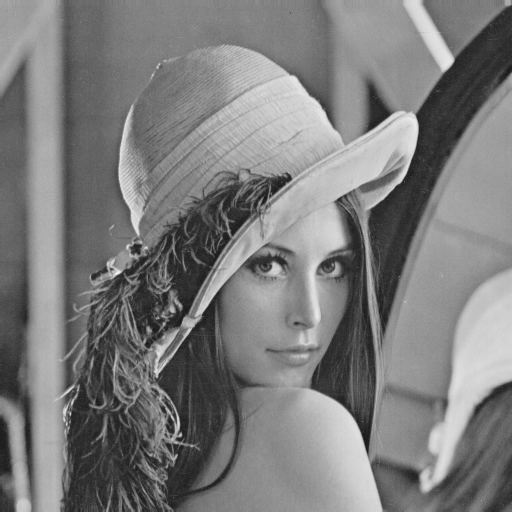
\includegraphics[height=9cm]{ej1-imgs/lena-original.png}
  \caption{\texttt{lena.png}}
\end{figure}

\begin{figure}[H]
\centering
\begin{subfigure}{0.5\linewidth}
\centering
  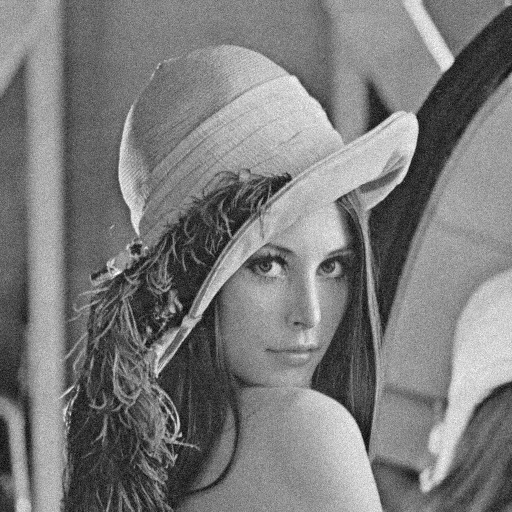
\includegraphics[height=9cm]{ej1-imgs/lena-gauss10.png}
  \caption{\footnotesize{\texttt{lena.png} con ruido gaussiano de media 10.}}
\end{subfigure}%
\begin{subfigure}{0.5\linewidth}
\centering
  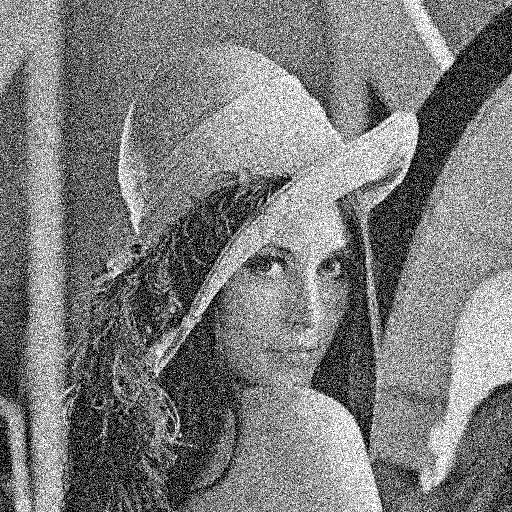
\includegraphics[height=9cm]{ej1-imgs/lena-gauss50.png}
  \caption{\footnotesize{\texttt{lena.png} con ruido gaussiano de media 50.}}
\end{subfigure}
\end{figure}

\begin{figure}[H]
\centering
\begin{subfigure}{0.5\linewidth}
\centering
  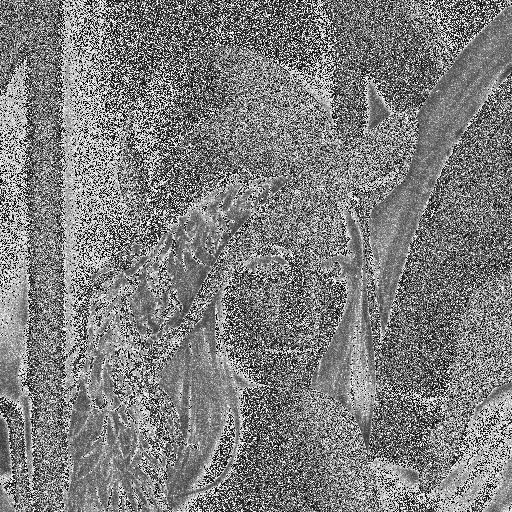
\includegraphics[height=9cm]{ej1-imgs/lena-rayleigh15.png}
  \caption{\footnotesize{\texttt{lena.png} con ruido rayleigh de parámetro 1.5.}}
\end{subfigure}%
\begin{subfigure}{0.5\linewidth}
\centering
  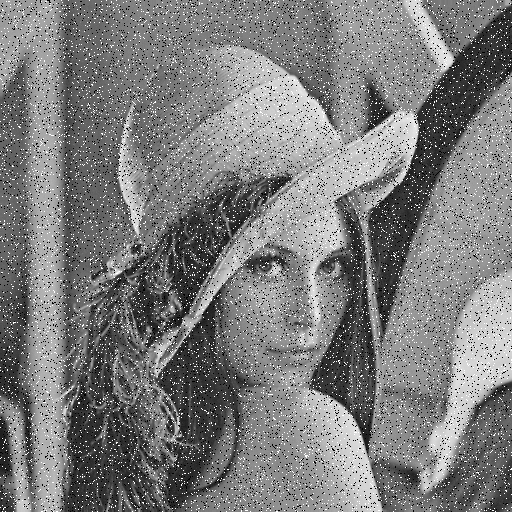
\includegraphics[height=9cm]{ej1-imgs/lena-saltpepper10.png}
  \caption{\footnotesize{\texttt{lena.png} con ruido salt \& pepper con probabilidad 0.1}}
\end{subfigure}
\end{figure}


\begin{figure}[H]
\centering
  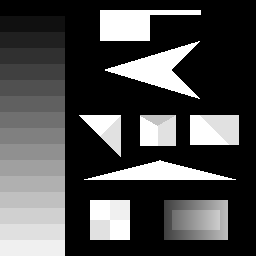
\includegraphics[height=9cm]{ej1-imgs/test-original.png}
  \caption{\texttt{test.png}}
\end{figure}

\begin{figure}[H]
\centering
\begin{subfigure}{0.5\linewidth}
\centering
  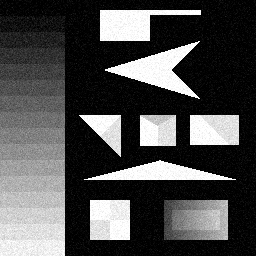
\includegraphics[height=9cm]{ej1-imgs/test-gauss10.png}
  \caption{\footnotesize{\texttt{test.png} con ruido gaussiano de media 10.}}
\end{subfigure}%
\begin{subfigure}{0.5\linewidth}
\centering
  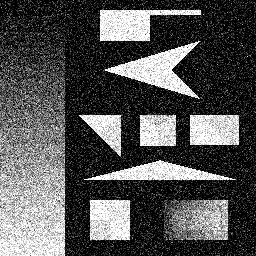
\includegraphics[height=9cm]{ej1-imgs/test-gauss50.png}
  \caption{\footnotesize{\texttt{test.png} con ruido gaussiano de media 50.}}
\end{subfigure}
\end{figure}

\begin{figure}[H]
\centering
\begin{subfigure}{0.5\linewidth}
\centering
  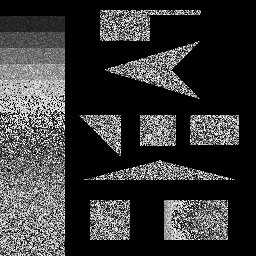
\includegraphics[height=9cm]{ej1-imgs/test-rayleigh15.png}
  \caption{\footnotesize{\texttt{test.png} con ruido rayleigh de parámetro 1.5.}}
\end{subfigure}%
\begin{subfigure}{0.5\linewidth}
\centering
  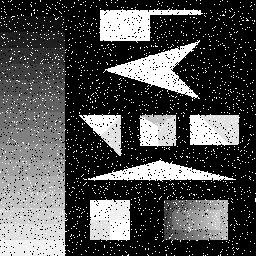
\includegraphics[height=9cm]{ej1-imgs/test-saltpepper10.png}
  \caption{\footnotesize{\texttt{test.png} con ruido salt \& pepper con probabilidad 0.1}}
\end{subfigure}
\end{figure}


\newpage
\section{Ejercicio 2: Métodos del Laplaciano}

Modo de uso
\begin{verbatim}
    python3 practica6/ej2.py <img> <a|b|c>
\end{verbatim}


\newpage
\subsection{a) Método del Laplaciano}

Este método se basa en calcular el laplaciano de la imágen, que es la suma de las derivadas segundas en cada dirección.
Luego, para detectar bordes, lo que se hace  es buscar en que píxeles el laplaciano cambia de signo, o sea, se buscan ceros (por eso el método se llama zero-crossing).

Además, no nos vamos a quedar con cualquier zero-crossing, si no aquellos que en la dirección del zero crossing la pendiente sea mayor que un límite (que será el doble de la mediana de todas las diferencias de los píxeles).

Como veremos a continuación, el filtro funciona bastante bien, pero se encuentra con problemas cuando hay mucho ruido en la imagen, porque la mediana de las diferencias  será muy grande y su valor será poco significativo para saber cuando un zero-crossing es interesante y cuando no.


\begin{figure}[H]
\centering
    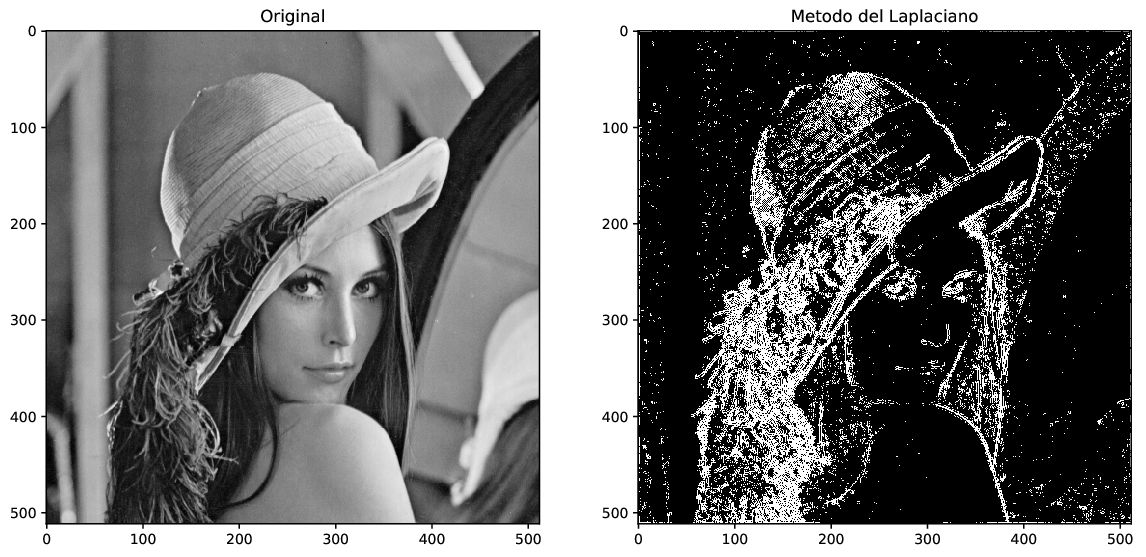
\includegraphics[height=6.5cm]{informe-imgs/ej2-a-lena-original.jpg}
    \caption{\texttt{python3 practica6/ej2.py practica6/ej1-imgs/lena-original.png a}}
\end{figure}

\begin{figure}[H]
\centering
    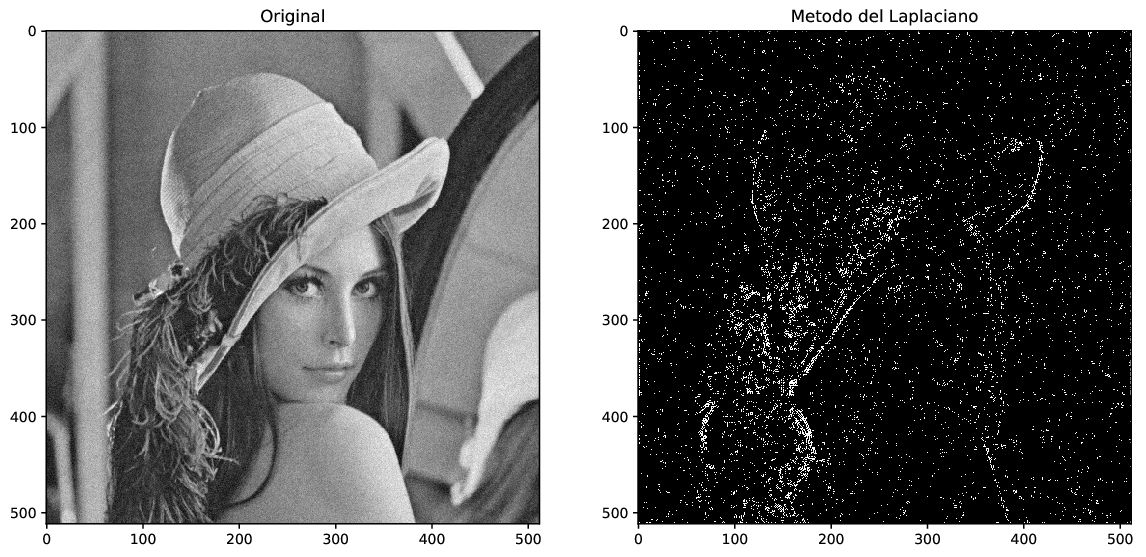
\includegraphics[height=6.5cm]{informe-imgs/ej2-a-lena-gauss10.jpg}
    \caption{\texttt{python3 practica6/ej2.py practica6/ej1-imgs/lena-gauss10.png a}}
\end{figure}

\begin{figure}[H]
\centering
    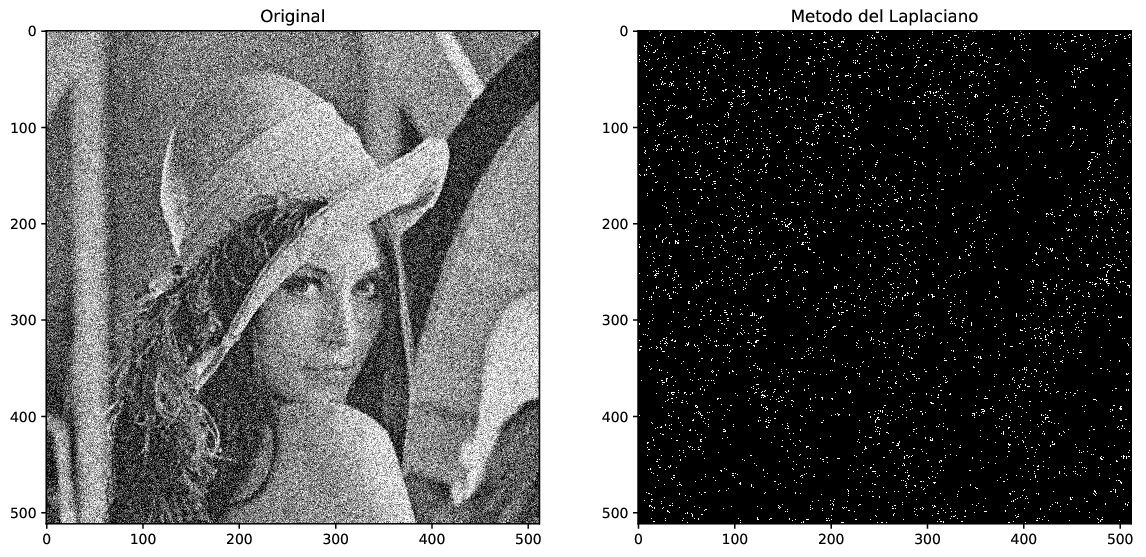
\includegraphics[height=6.5cm]{informe-imgs/ej2-a-lena-gauss50.jpg}
    \caption{\texttt{python3 practica6/ej2.py practica6/ej1-imgs/lena-gauss50.png a}}
\end{figure}

\begin{figure}[H]
\centering
    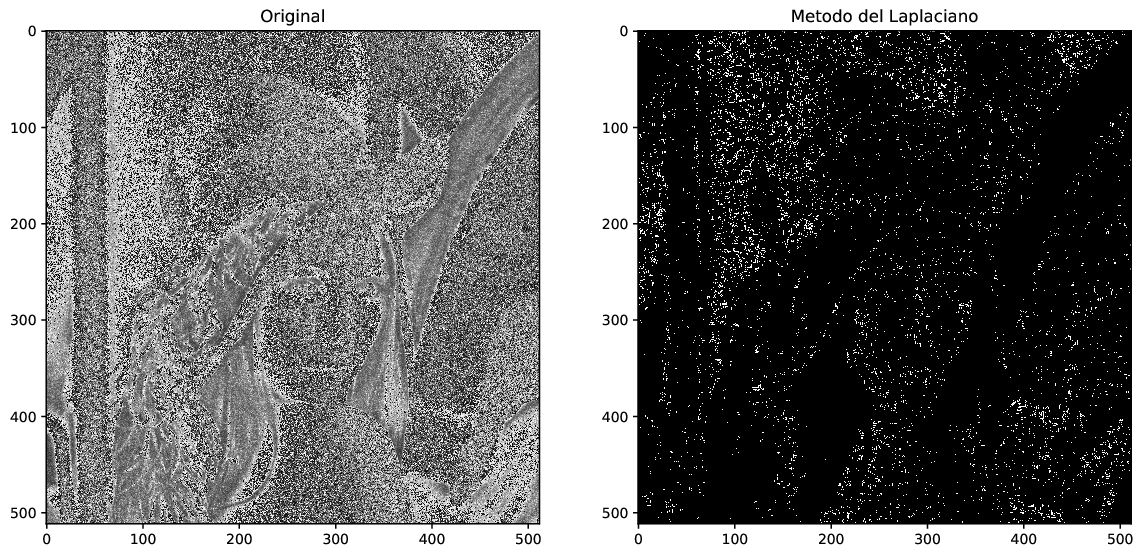
\includegraphics[height=6.5cm]{informe-imgs/ej2-a-lena-rayleigh15.jpg}
    \caption{\texttt{python3 practica6/ej2.py practica6/ej1-imgs/lena-rayleigh15.png a}}
\end{figure}

\begin{figure}[H]
\centering
    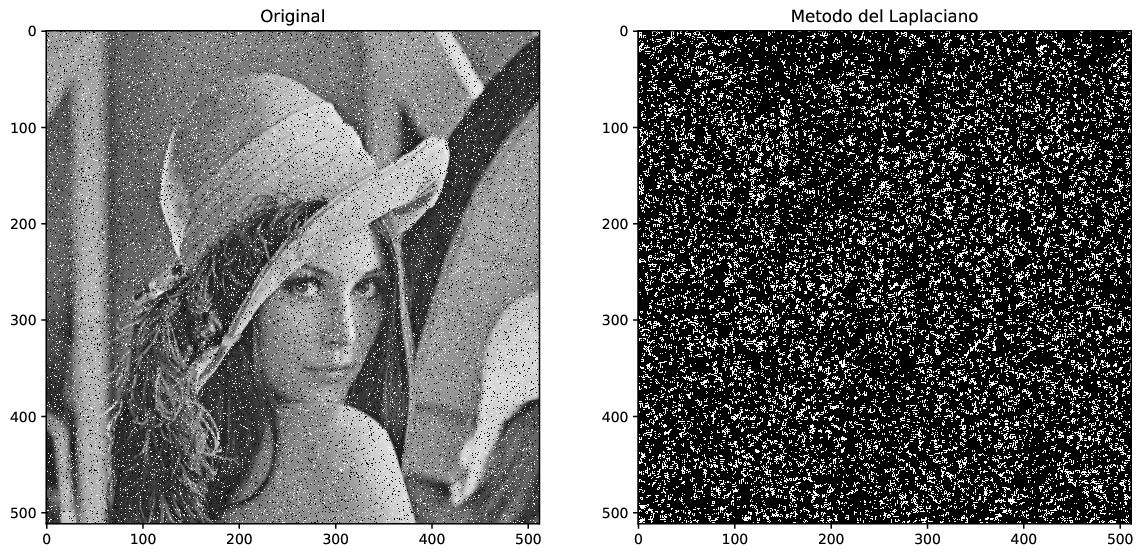
\includegraphics[height=6.5cm]{informe-imgs/ej2-a-lena-saltpepper10.jpg}
    \caption{\texttt{python3 practica6/ej2.py practica6/ej1-imgs/lena-saltpepper10.png a}}
\end{figure}


\begin{figure}[H]
\centering
    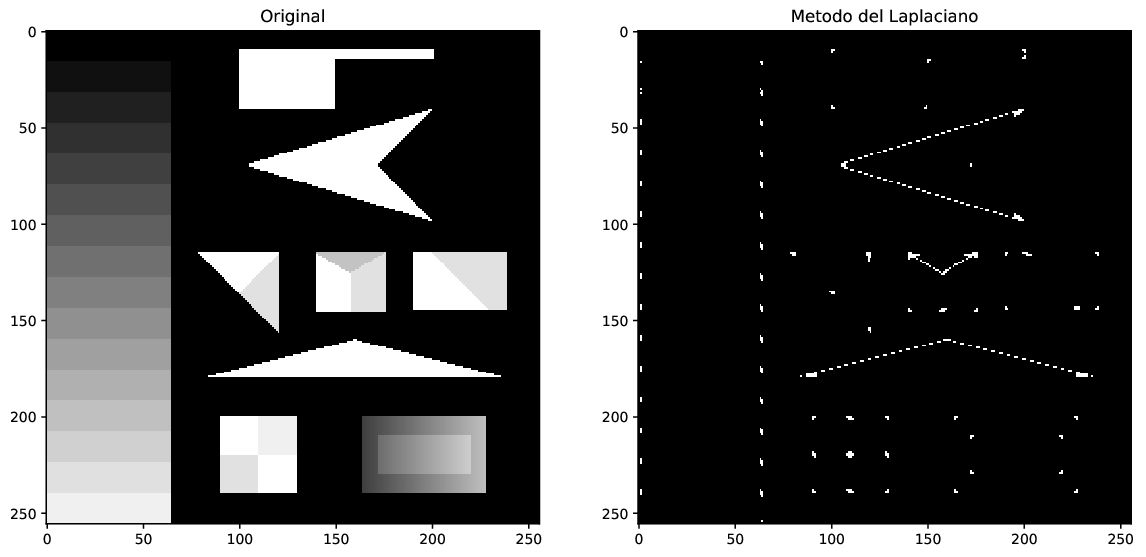
\includegraphics[height=6.5cm]{informe-imgs/ej2-a-test-original.jpg}
    \caption{\texttt{python3 practica6/ej2.py practica6/ej1-imgs/test-original.png a}}
\end{figure}

\begin{figure}[H]
\centering
    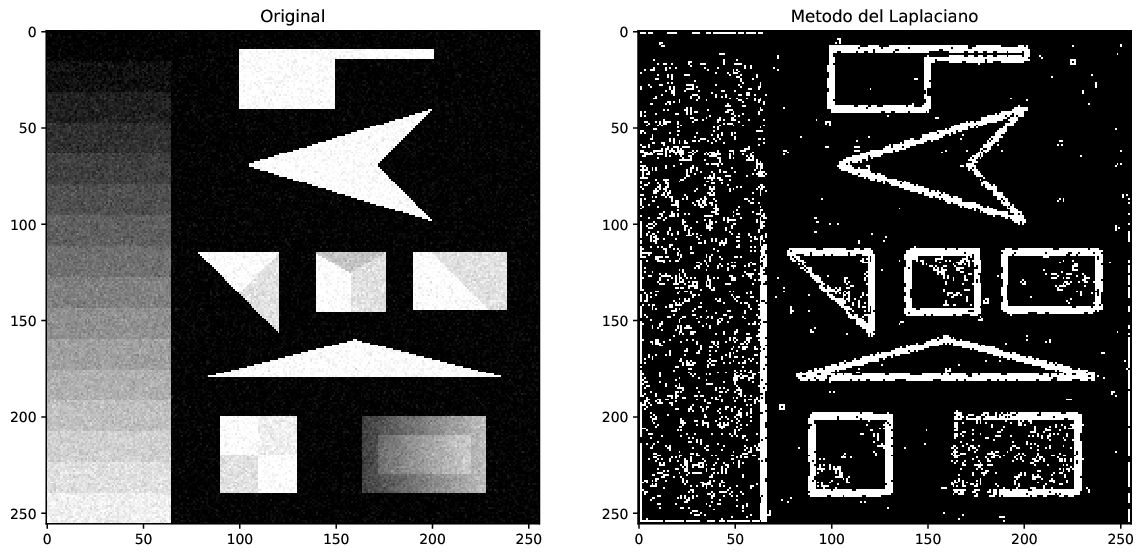
\includegraphics[height=6.5cm]{informe-imgs/ej2-a-test-gauss10.jpg}
    \caption{\texttt{python3 practica6/ej2.py practica6/ej1-imgs/test-gauss10.png a}}
\end{figure}

\begin{figure}[H]
\centering
    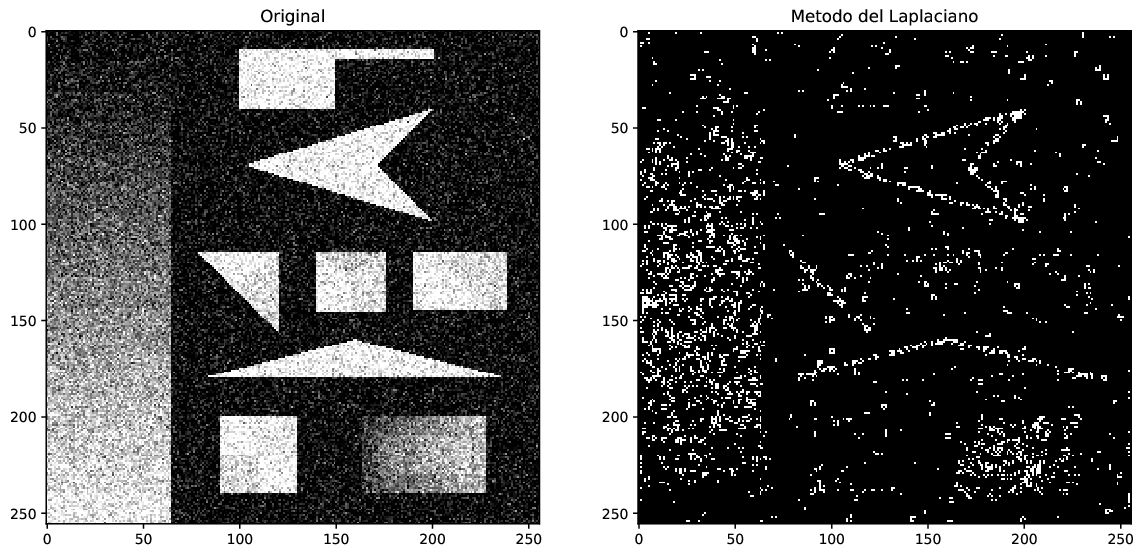
\includegraphics[height=6.5cm]{informe-imgs/ej2-a-test-gauss50.jpg}
    \caption{\texttt{python3 practica6/ej2.py practica6/ej1-imgs/test-gauss50.png a}}
\end{figure}

\begin{figure}[H]
\centering
    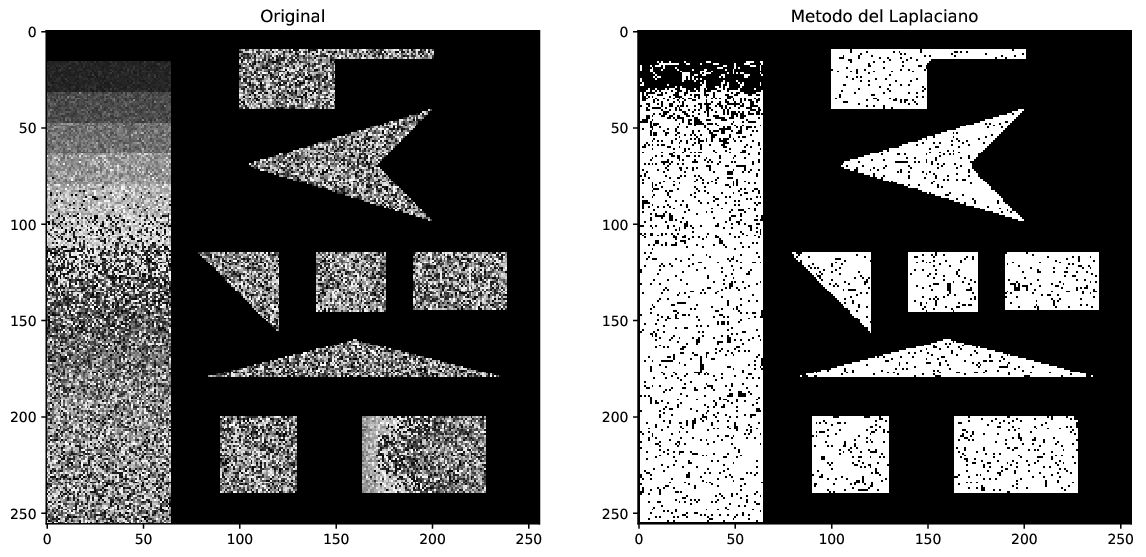
\includegraphics[height=6.5cm]{informe-imgs/ej2-a-test-rayleigh15.jpg}
    \caption{\texttt{python3 practica6/ej2.py practica6/ej1-imgs/test-rayleigh15.png a}}
\end{figure}

\begin{figure}[H]
\centering
    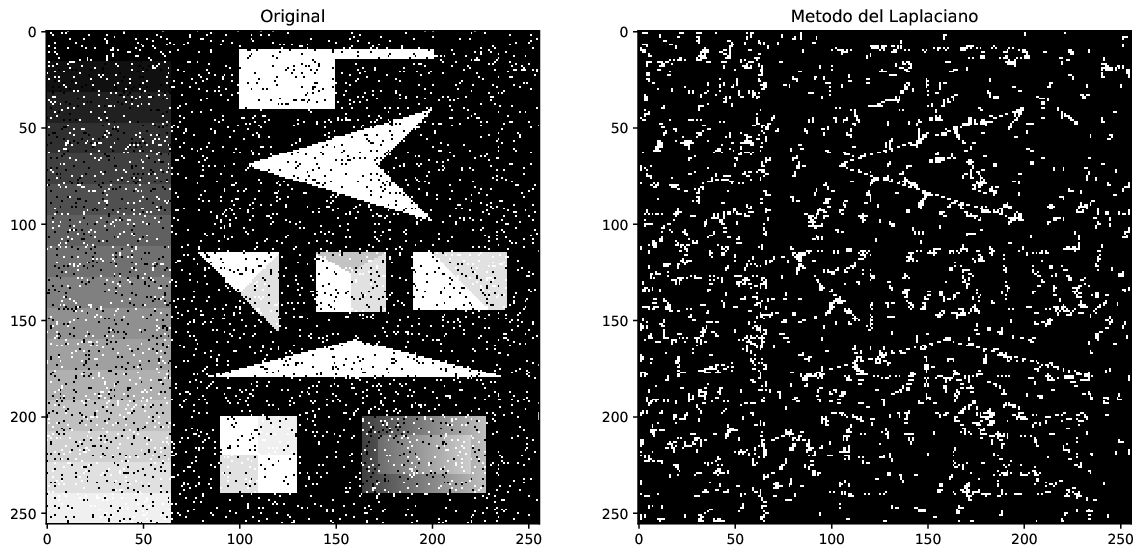
\includegraphics[height=6.5cm]{informe-imgs/ej2-a-test-saltpepper10.jpg}
    \caption{\texttt{python3 practica6/ej2.py practica6/ej1-imgs/test-saltpepper10.png a}}
\end{figure}


\newpage
\subsection{b) Método del Laplaciano con evaluación local de varianza}

Este método es muy parecido al anterior, solo que para decidir si un zero-crossing se corresponde con un borde, miraremos la varianza del vecindario del pixel.

La varianza del vecindario del pixel es la raiz cuadrada de la suma del cuadrado de las diferencias, dividido por la cantidad de elementos del vecindario.

Si esta cuenta da mayor que 2, diremos que el pixel en cuestión es un borde, si no no.

Como se nota en los resultados, para aquellas imágenes con mucho ruido la detección de bordes mejora, pero sólo marginalmente.


\begin{figure}[H]
\centering
    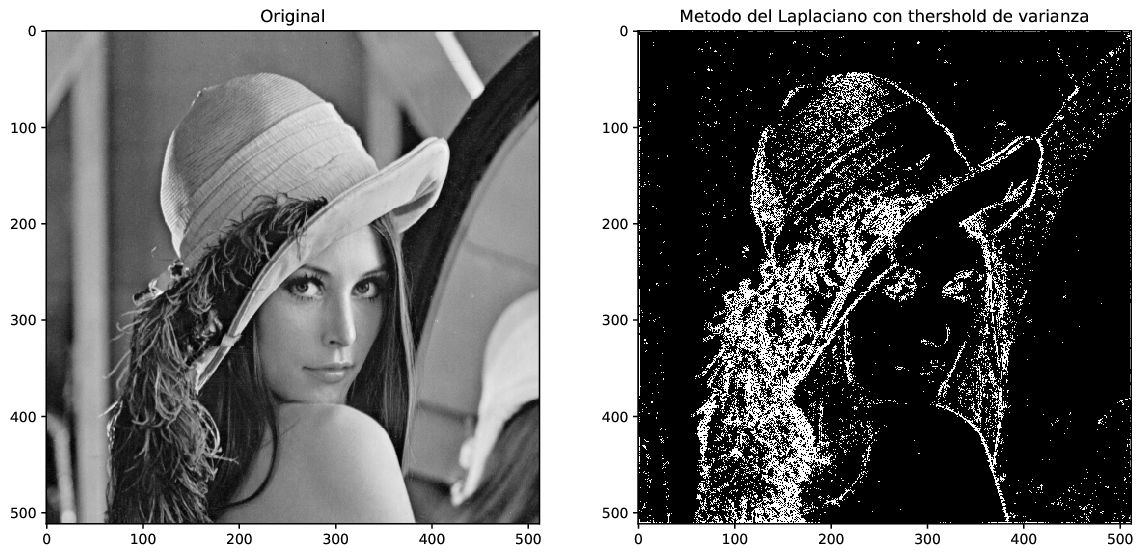
\includegraphics[height=6.5cm]{informe-imgs/ej2-b-lena-original.jpg}
    \caption{\texttt{python3 practica6/ej2.py practica6/ej1-imgs/lena-original.png b}}
\end{figure}

\begin{figure}[H]
\centering
    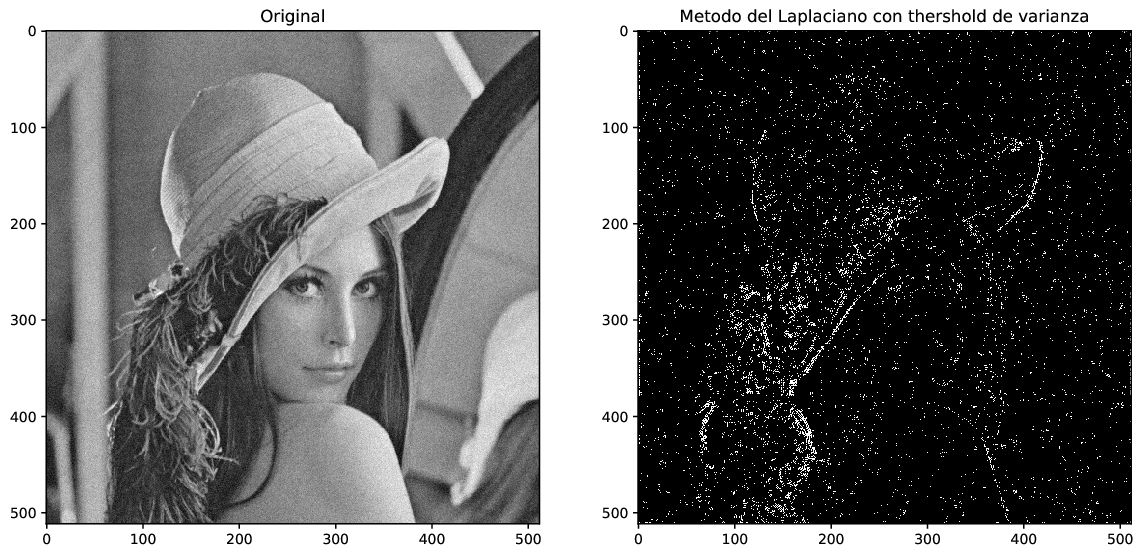
\includegraphics[height=6.5cm]{informe-imgs/ej2-b-lena-gauss10.jpg}
    \caption{\texttt{python3 practica6/ej2.py practica6/ej1-imgs/lena-gauss10.png b}}
\end{figure}

\begin{figure}[H]
\centering
    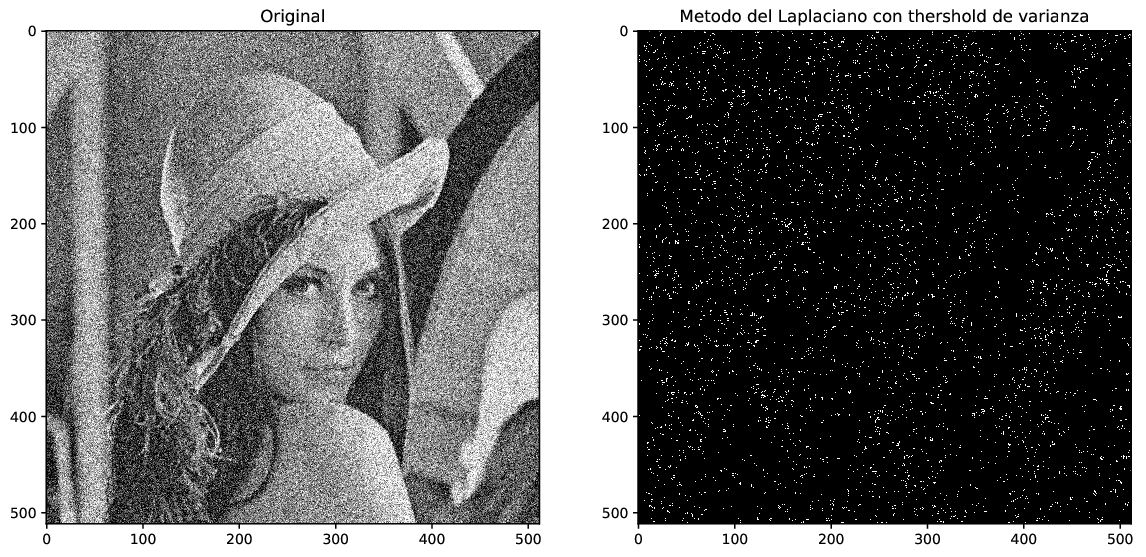
\includegraphics[height=6.5cm]{informe-imgs/ej2-b-lena-gauss50.jpg}
    \caption{\texttt{python3 practica6/ej2.py practica6/ej1-imgs/lena-gauss50.png b}}
\end{figure}

\begin{figure}[H]
\centering
    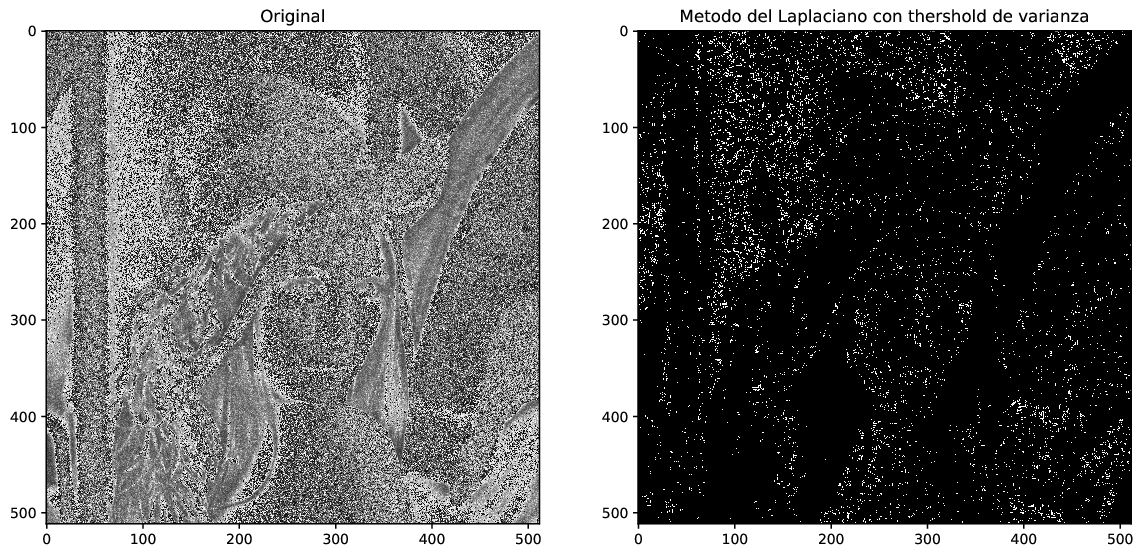
\includegraphics[height=6.5cm]{informe-imgs/ej2-b-lena-rayleigh15.jpg}
    \caption{\texttt{python3 practica6/ej2.py practica6/ej1-imgs/lena-rayleigh15.png b}}
\end{figure}

\begin{figure}[H]
\centering
    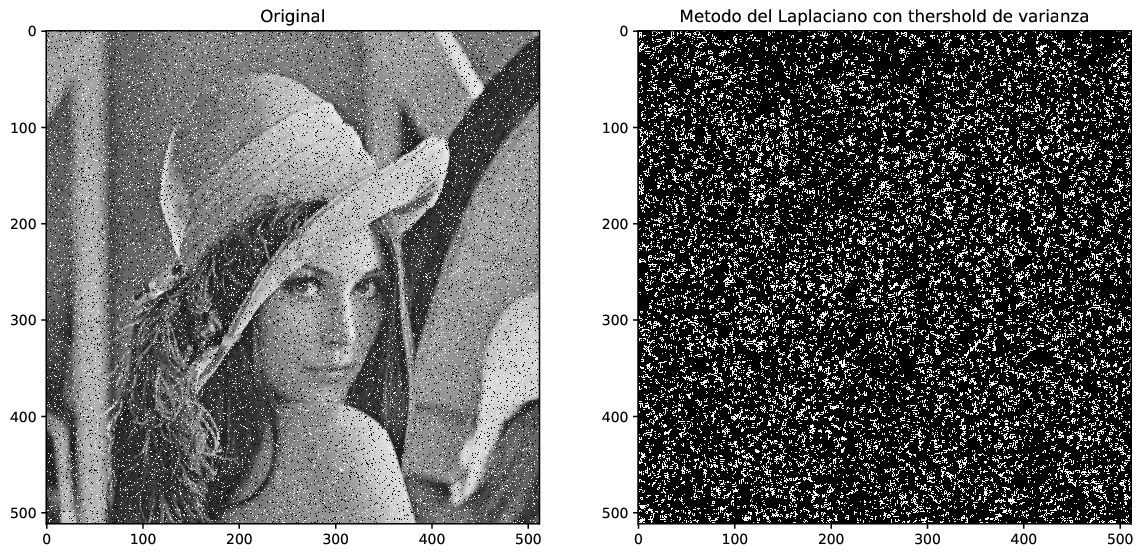
\includegraphics[height=6.5cm]{informe-imgs/ej2-b-lena-saltpepper10.jpg}
    \caption{\texttt{python3 practica6/ej2.py practica6/ej1-imgs/lena-saltpepper10.png b}}
\end{figure}


\begin{figure}[H]
\centering
    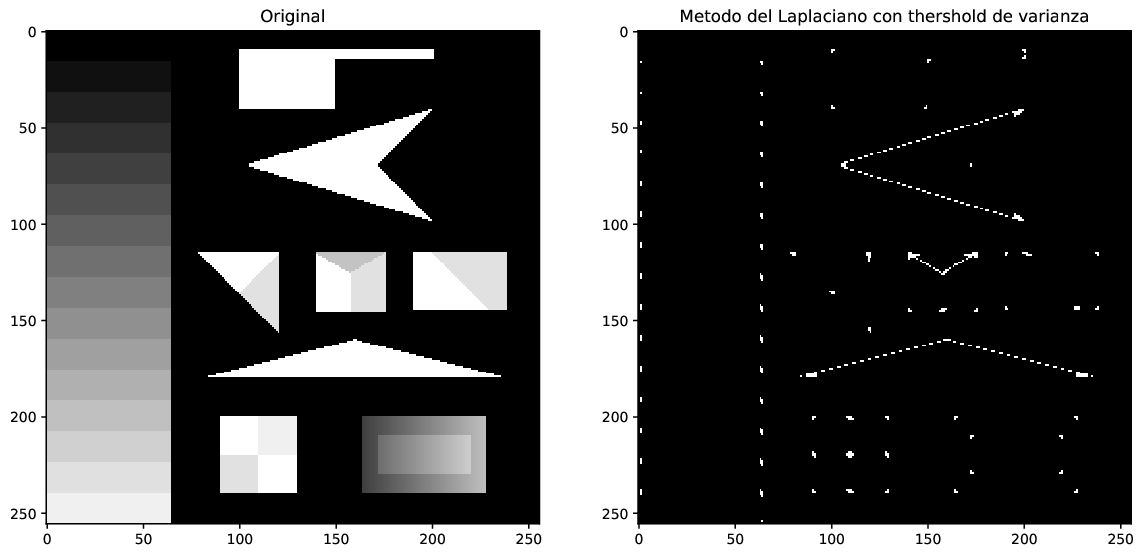
\includegraphics[height=6.5cm]{informe-imgs/ej2-b-test-original.jpg}
    \caption{\texttt{python3 practica6/ej2.py practica6/ej1-imgs/test-original.png b}}
\end{figure}

\begin{figure}[H]
\centering
    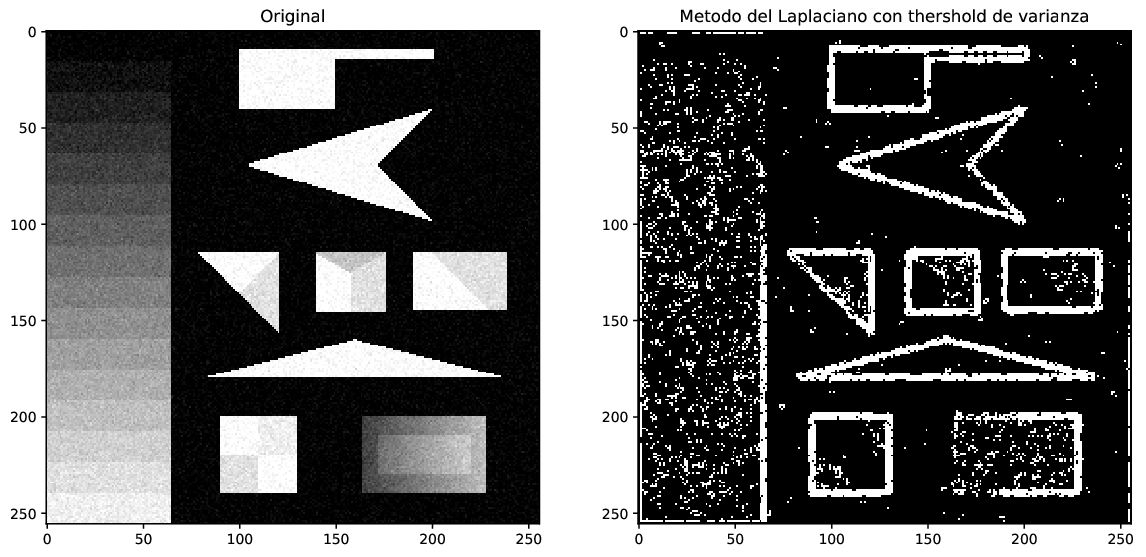
\includegraphics[height=6.5cm]{informe-imgs/ej2-b-test-gauss10.jpg}
    \caption{\texttt{python3 practica6/ej2.py practica6/ej1-imgs/test-gauss10.png b}}
\end{figure}

\begin{figure}[H]
\centering
    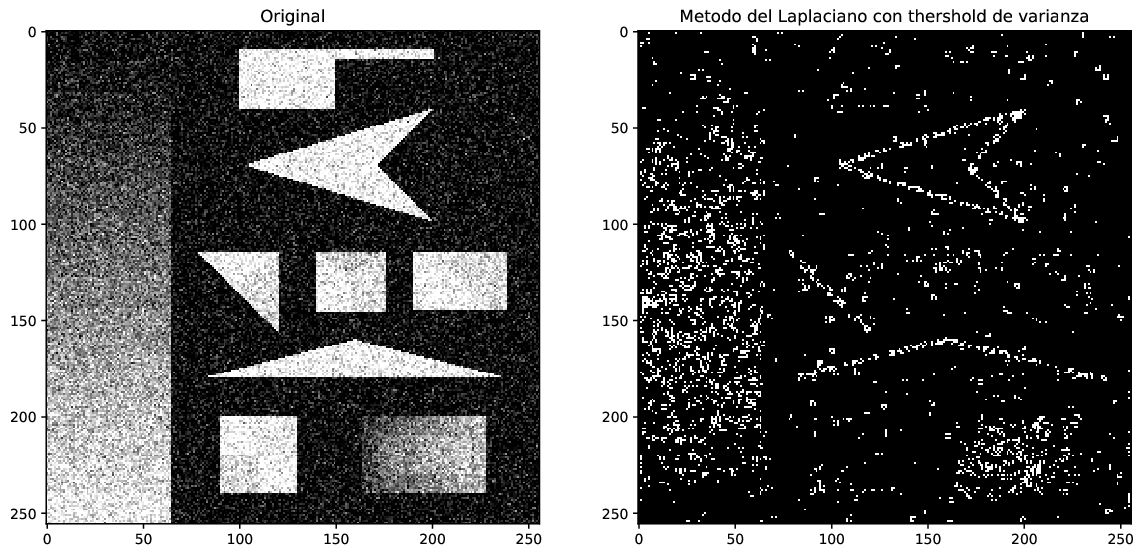
\includegraphics[height=6.5cm]{informe-imgs/ej2-b-test-gauss50.jpg}
    \caption{\texttt{python3 practica6/ej2.py practica6/ej1-imgs/test-gauss50.png b}}
\end{figure}

\begin{figure}[H]
\centering
    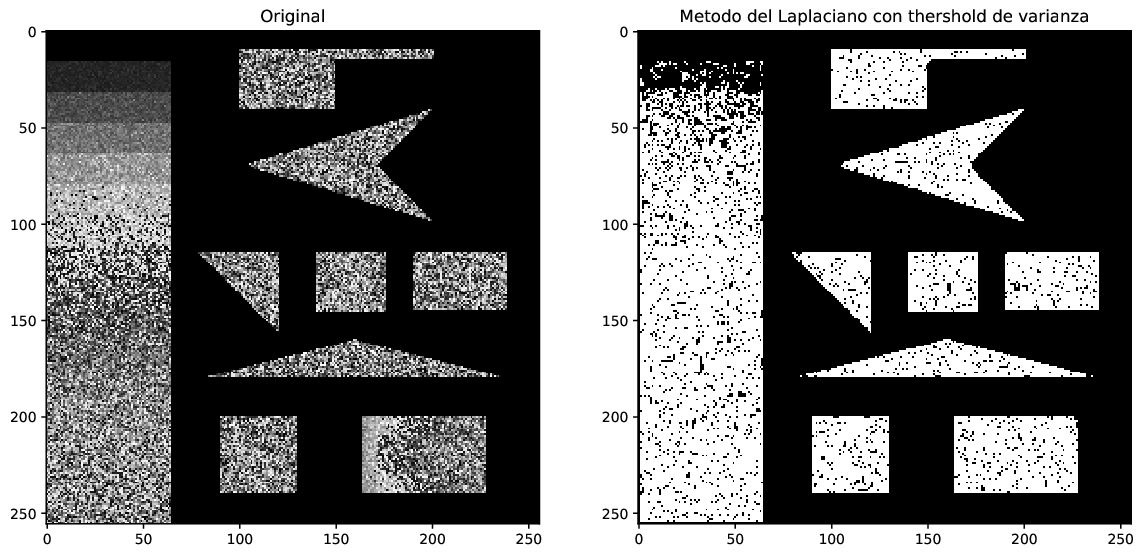
\includegraphics[height=6.5cm]{informe-imgs/ej2-b-test-rayleigh15.jpg}
    \caption{\texttt{python3 practica6/ej2.py practica6/ej1-imgs/test-rayleigh15.png b}}
\end{figure}

\begin{figure}[H]
\centering
    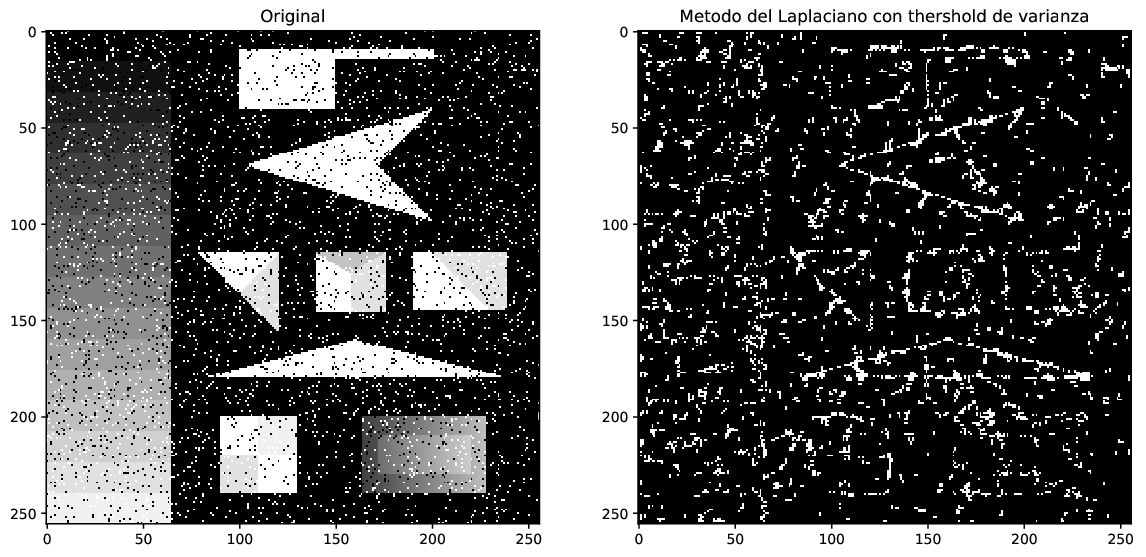
\includegraphics[height=6.5cm]{informe-imgs/ej2-b-test-saltpepper10.jpg}
    \caption{\texttt{python3 practica6/ej2.py practica6/ej1-imgs/test-saltpepper10.png b}}
\end{figure}


\newpage
\subsection{c) Método del Laplaciano del Gaussiano}

Este es otro método que apunta a detectar bordes en imágenes con ruido. La idea es usar el método del laplaciano del primer ejercicio, pero antes pasarle a la imágen un filtro que la difumine, en este caso un filtro gaussiano.
Esto apunta a reducir el ruido y trabajar con una imagen que se preste más al análisis de zero-crossing.

Como puede apreciarse, los resultados son muchísimo mejores, sobre todo en las imágenes de test.png, en la cual en todos los casos pueden detectarse los bordes, aún con mucho ruido.

\begin{figure}[H]
\centering
    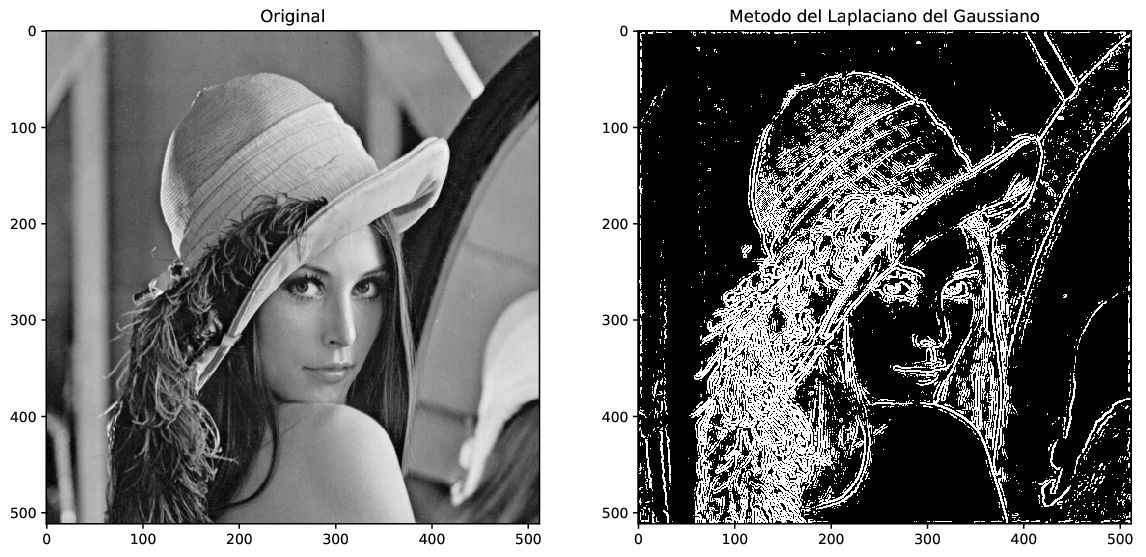
\includegraphics[height=6.5cm]{informe-imgs/ej2-c-lena-original.jpg}
    \caption{\texttt{python3 practica6/ej2.py practica6/ej1-imgs/lena-original.png c}}
\end{figure}

\begin{figure}[H]
\centering
    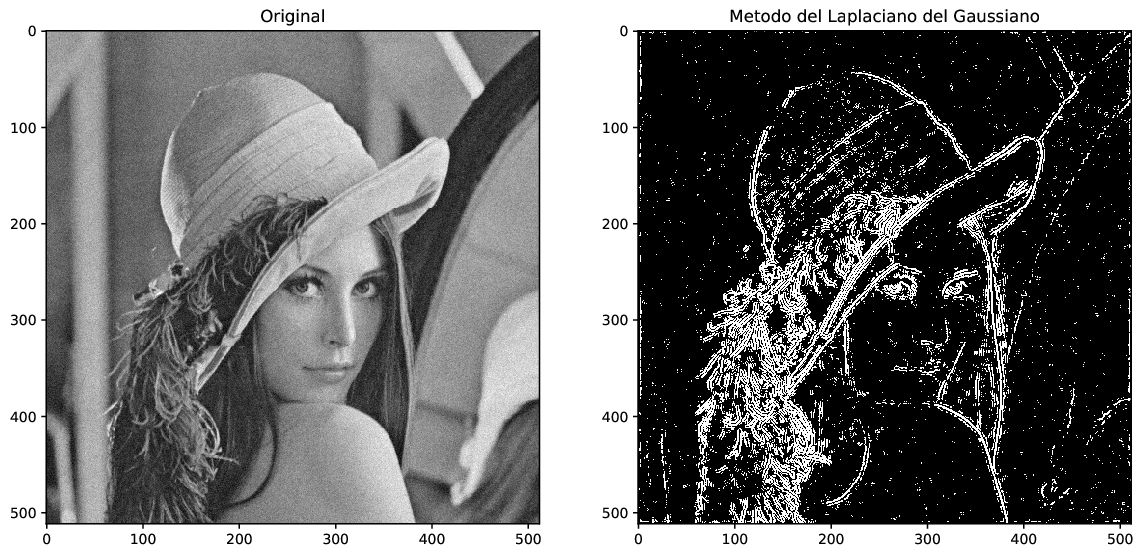
\includegraphics[height=6.5cm]{informe-imgs/ej2-c-lena-gauss10.jpg}
    \caption{\texttt{python3 practica6/ej2.py practica6/ej1-imgs/lena-gauss10.png c}}
\end{figure}

\begin{figure}[H]
\centering
    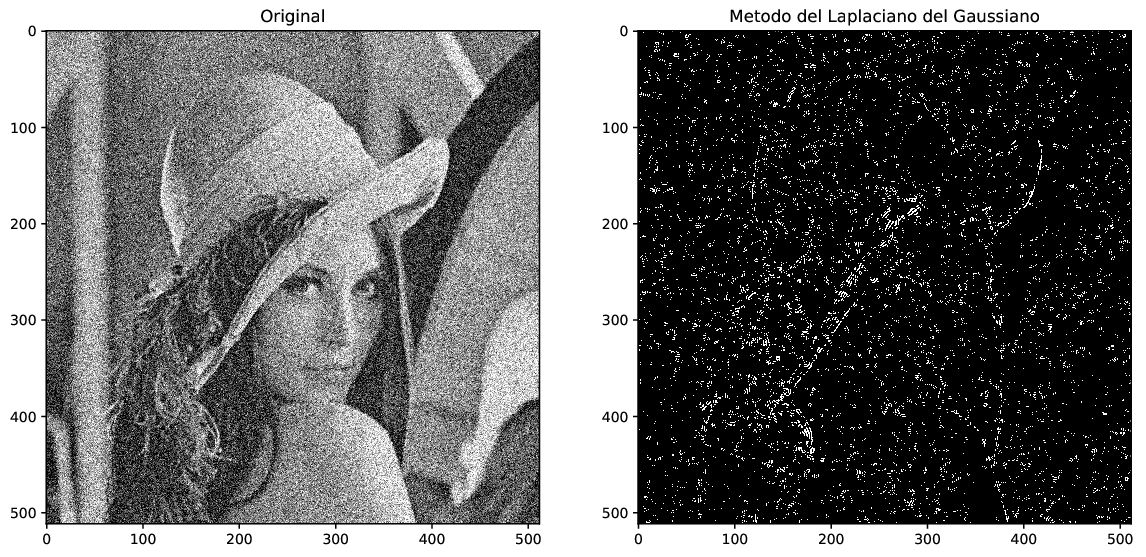
\includegraphics[height=6.5cm]{informe-imgs/ej2-c-lena-gauss50.jpg}
    \caption{\texttt{python3 practica6/ej2.py practica6/ej1-imgs/lena-gauss50.png c}}
\end{figure}

\begin{figure}[H]
\centering
    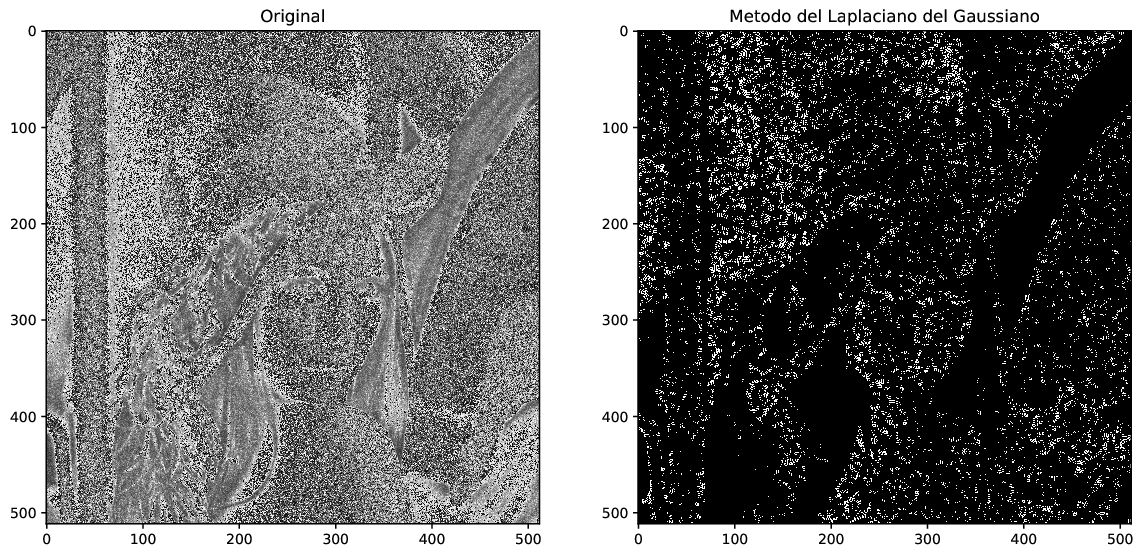
\includegraphics[height=6.5cm]{informe-imgs/ej2-c-lena-rayleigh15.jpg}
    \caption{\texttt{python3 practica6/ej2.py practica6/ej1-imgs/lena-rayleigh15.png c}}
\end{figure}

\begin{figure}[H]
\centering
    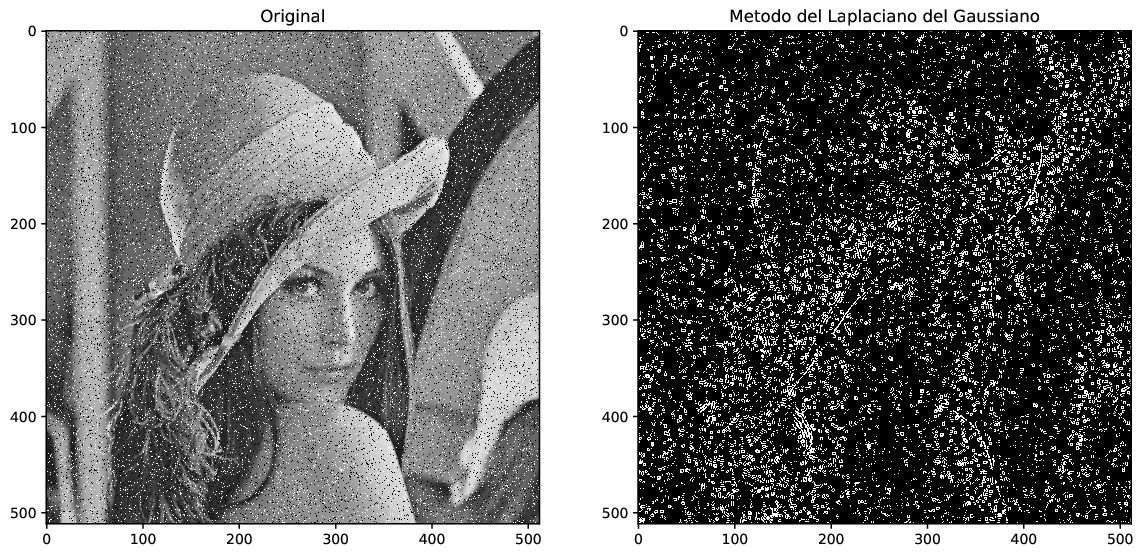
\includegraphics[height=6.5cm]{informe-imgs/ej2-c-lena-saltpepper10.jpg}
    \caption{\texttt{python3 practica6/ej2.py practica6/ej1-imgs/lena-saltpepper10.png c}}
\end{figure}


\begin{figure}[H]
\centering
    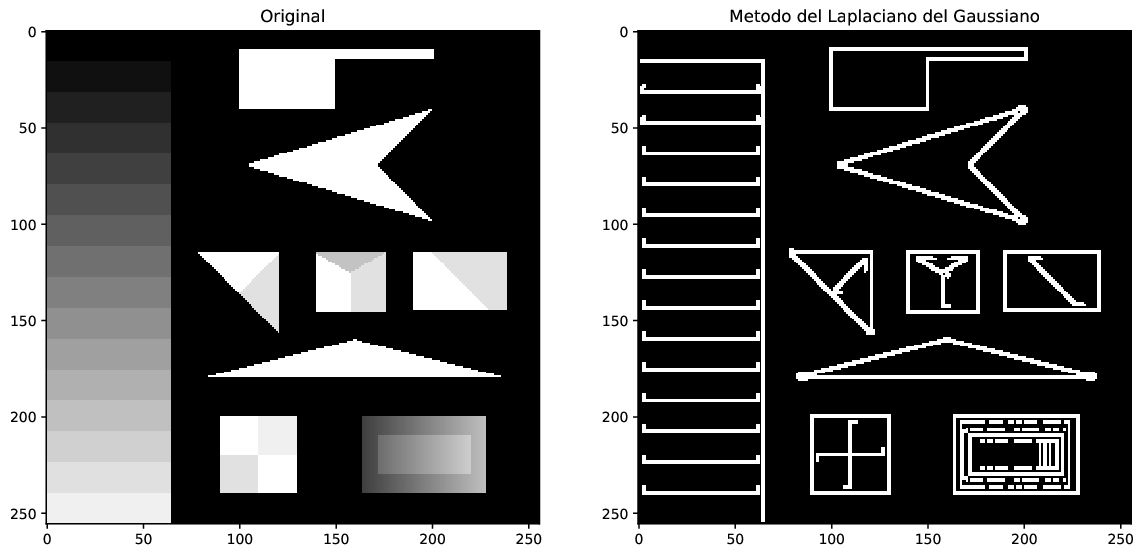
\includegraphics[height=6.5cm]{informe-imgs/ej2-c-test-original.jpg}
    \caption{\texttt{python3 practica6/ej2.py practica6/ej1-imgs/test-original.png c}}
\end{figure}

\begin{figure}[H]
\centering
    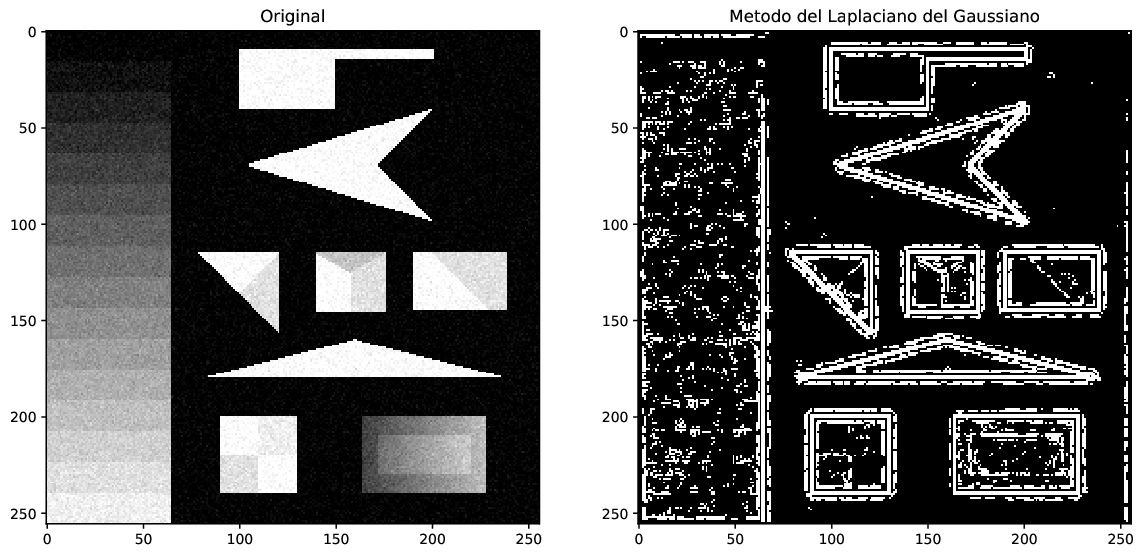
\includegraphics[height=6.5cm]{informe-imgs/ej2-c-test-gauss10.jpg}
    \caption{\texttt{python3 practica6/ej2.py practica6/ej1-imgs/test-gauss10.png c}}
\end{figure}

\begin{figure}[H]
\centering
    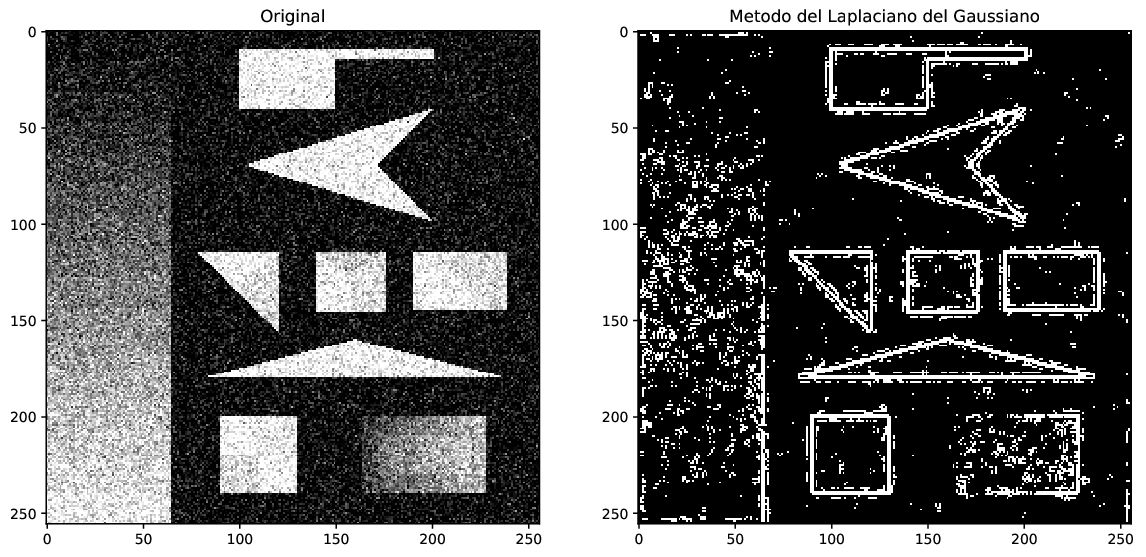
\includegraphics[height=6.5cm]{informe-imgs/ej2-c-test-gauss50.jpg}
    \caption{\texttt{python3 practica6/ej2.py practica6/ej1-imgs/test-gauss50.png c}}
\end{figure}

\begin{figure}[H]
\centering
    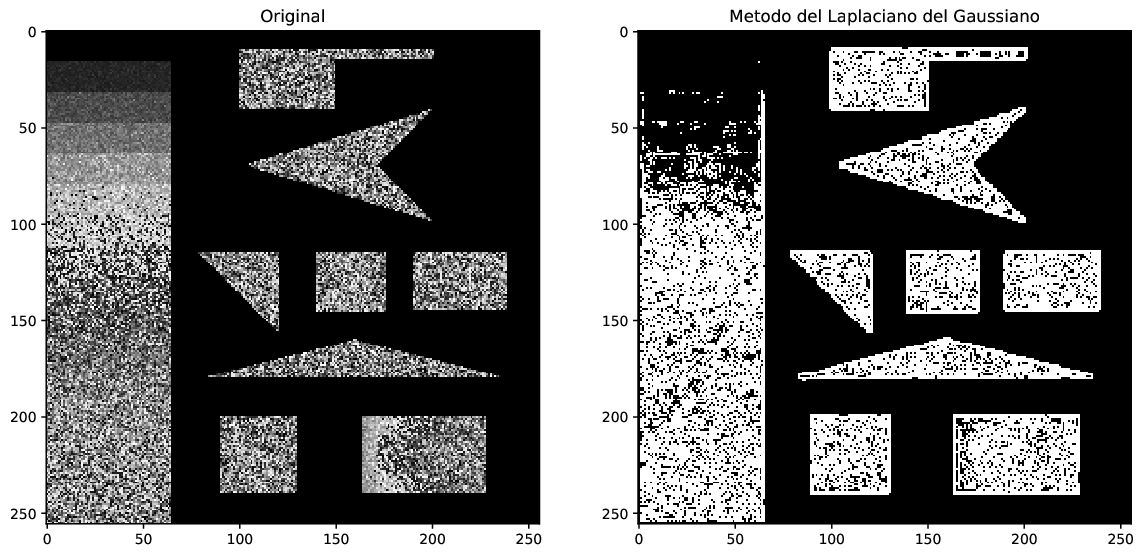
\includegraphics[height=6.5cm]{informe-imgs/ej2-c-test-rayleigh15.jpg}
    \caption{\texttt{python3 practica6/ej2.py practica6/ej1-imgs/test-rayleigh15.png c}}
\end{figure}

\begin{figure}[H]
\centering
    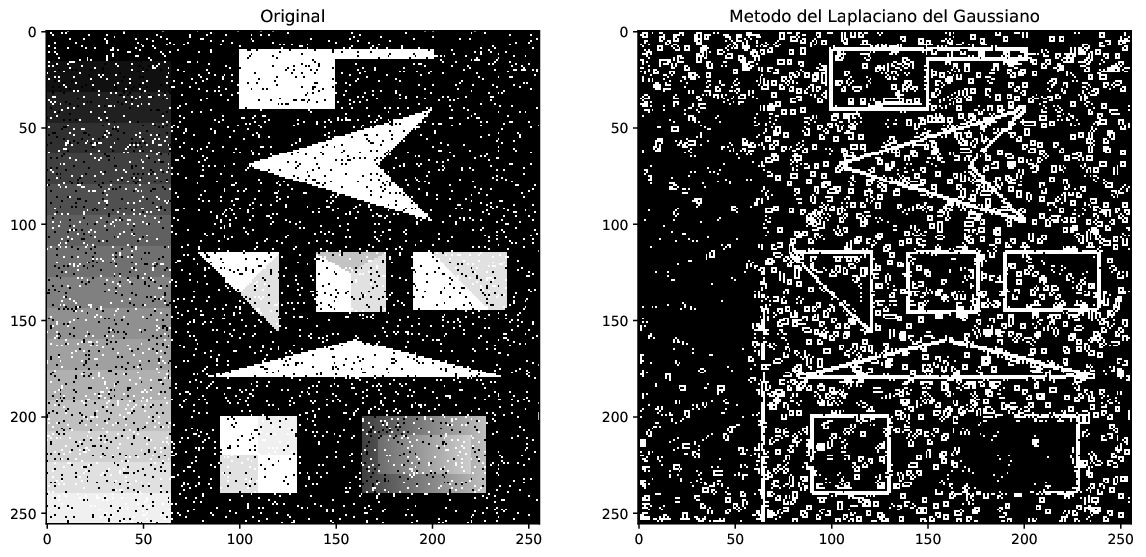
\includegraphics[height=6.5cm]{informe-imgs/ej2-c-test-saltpepper10.jpg}
    \caption{\texttt{python3 practica6/ej2.py practica6/ej1-imgs/test-saltpepper10.png c}}
\end{figure}

\newpage
\section{Ejercicio 3: Filtro de Kirsch}

Modo de uso
\begin{verbatim}
    python3 practica6/ej3.py <img>
\end{verbatim}

El filtro de Kirsch se basa en aplicar los siguientes operadores a la imágen y luego tomar el máximo entre todos ellos. Cada operador tiene una dirección, N, NE, E, SE, S, SO, O, NO. 

\[
\mathbf{g^{(1)}} = \begin{bmatrix} 
+5 & +5 & +5 \\
-3 &  0 & -3 \\
-3 & -3 & -3 
\end{bmatrix},\
\]
\[
\mathbf{g^{(2)}} = \begin{bmatrix} 
+5 & +5 & -3 \\
+5 &  0 & -3 \\
-3 & -3 & -3 
\end{bmatrix},\ 
\]
\[
\mathbf{g^{(3)}} = \begin{bmatrix} 
+5 & -3 & -3 \\
+5 &  0 & -3 \\
+5 & -3 & -3 
\end{bmatrix},\ 
\]
\[
\mathbf{g^{(4)}} = \begin{bmatrix} 
-3 & -3 & -3 \\
+5 &  0 & -3 \\
+5 & +5 & -3 
\end{bmatrix}
\]
\[
\vdots
\]

Como puede verse, los resultados son muy buenos en las imágenes originales. Sin embargo, para las imágenes con ruido los resultados son muy distintos. En lena, los resultados on muy pobres. Esto se debe a que los bordes de la imagen de lena con mucho ruido son casi indistinguibles. En cambio, en test, los bordes siguen siendo bastante distinguibles en la dirección en la que están, con lo cual funciona mucho mejor.

\begin{figure}[H]
\centering
    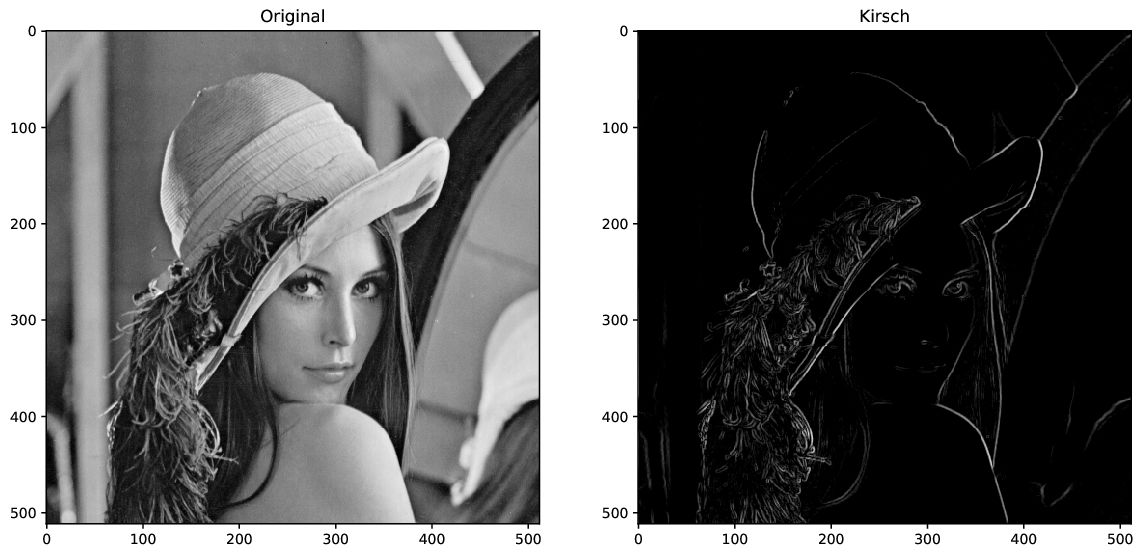
\includegraphics[height=6.5cm]{informe-imgs/ej3--lena-original.jpg}
    \caption{\texttt{python3 practica6/ej3.py practica6/ej1-imgs/lena-original.png }}
\end{figure}

\begin{figure}[H]
\centering
    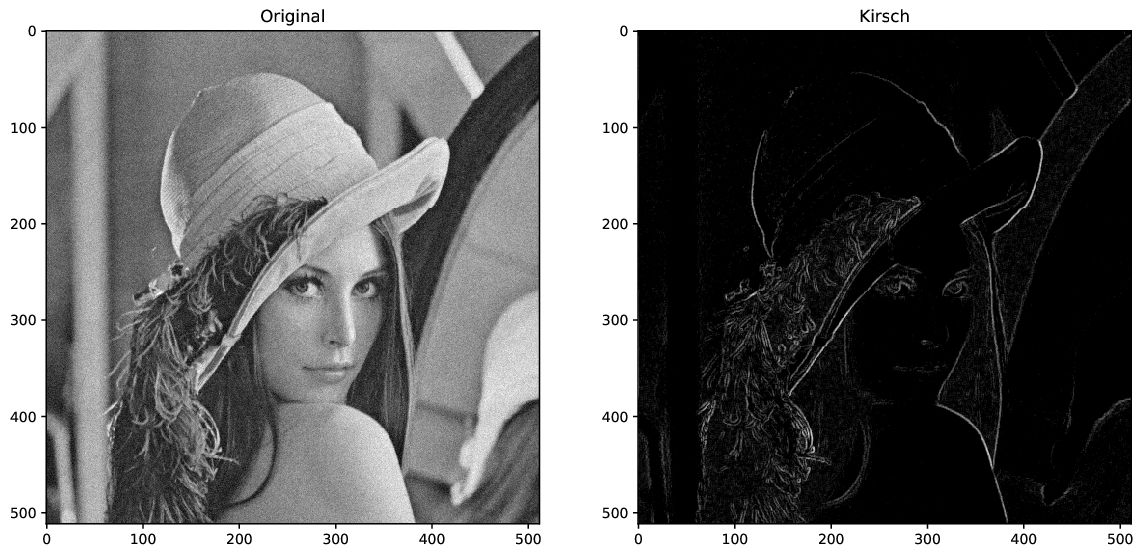
\includegraphics[height=6.5cm]{informe-imgs/ej3--lena-gauss10.jpg}
    \caption{\texttt{python3 practica6/ej3.py practica6/ej1-imgs/lena-gauss10.png }}
\end{figure}

\begin{figure}[H]
\centering
    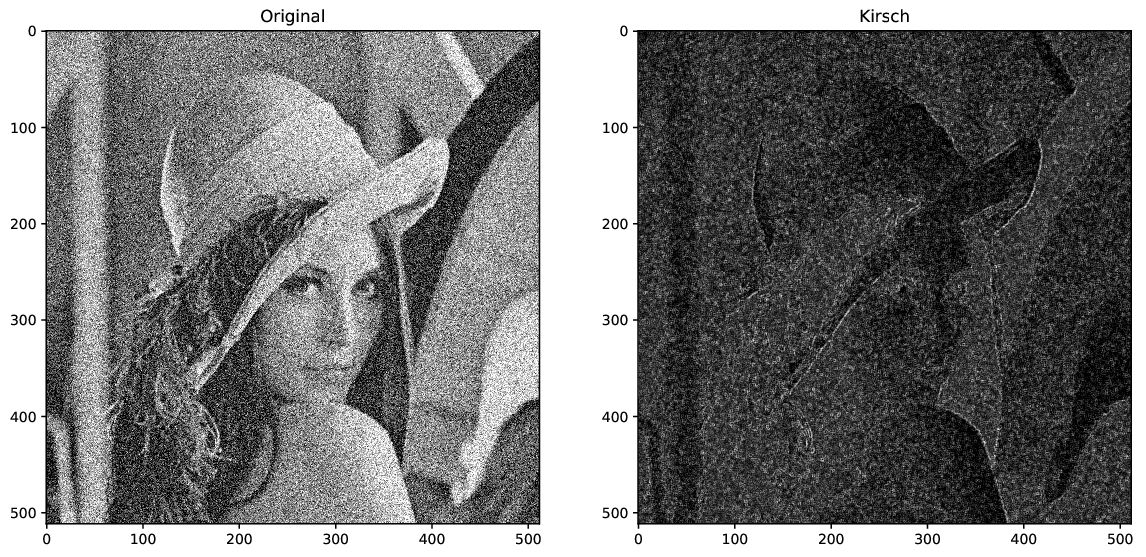
\includegraphics[height=6.5cm]{informe-imgs/ej3--lena-gauss50.jpg}
    \caption{\texttt{python3 practica6/ej3.py practica6/ej1-imgs/lena-gauss50.png }}
\end{figure}

\begin{figure}[H]
\centering
    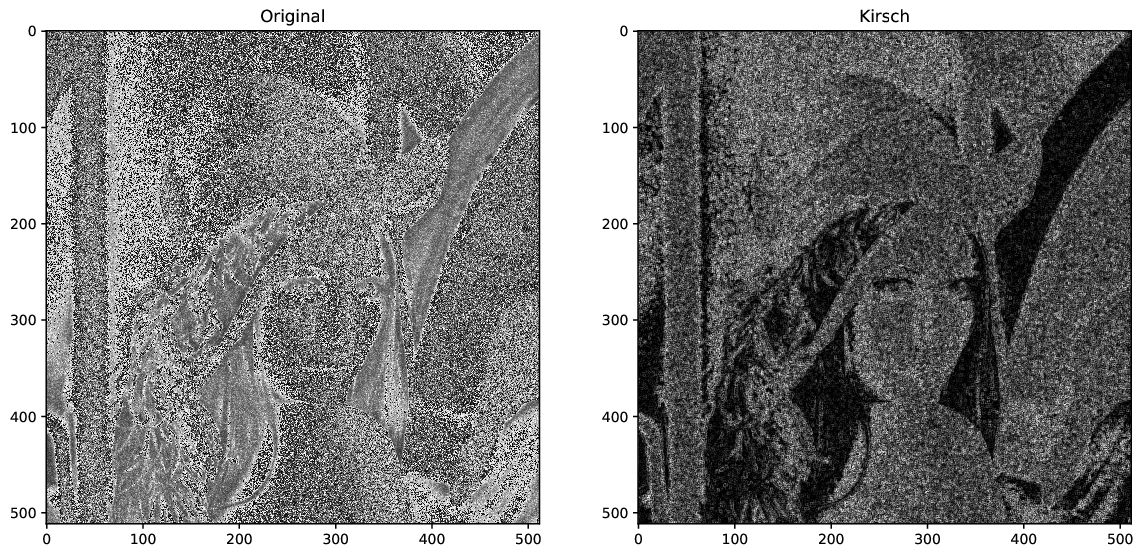
\includegraphics[height=6.5cm]{informe-imgs/ej3--lena-rayleigh15.jpg}
    \caption{\texttt{python3 practica6/ej3.py practica6/ej1-imgs/lena-rayleigh15.png }}
\end{figure}

\begin{figure}[H]
\centering
    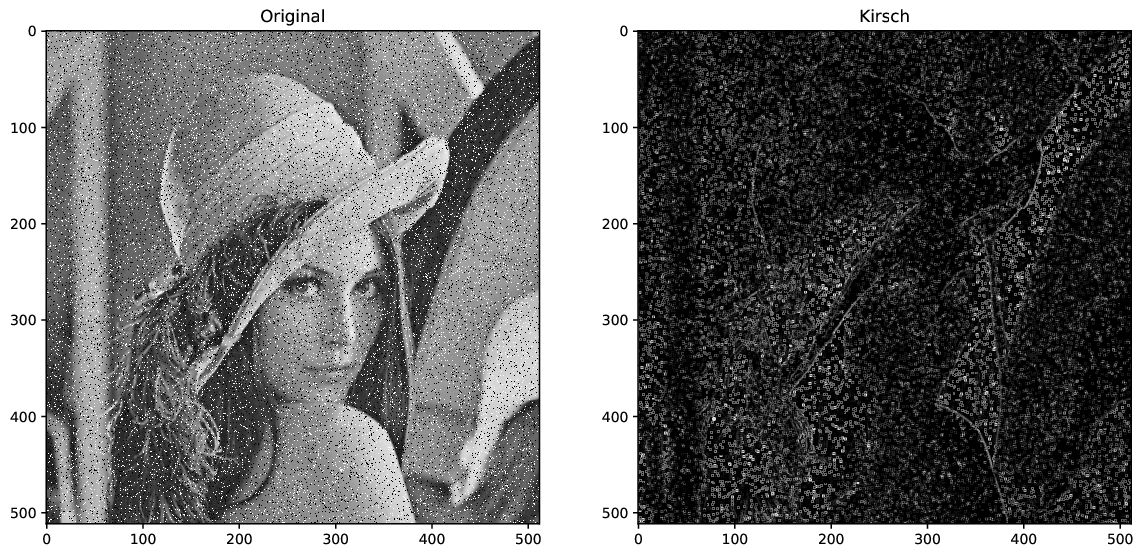
\includegraphics[height=6.5cm]{informe-imgs/ej3--lena-saltpepper10.jpg}
    \caption{\texttt{python3 practica6/ej3.py practica6/ej1-imgs/lena-saltpepper10.png }}
\end{figure}


\begin{figure}[H]
\centering
    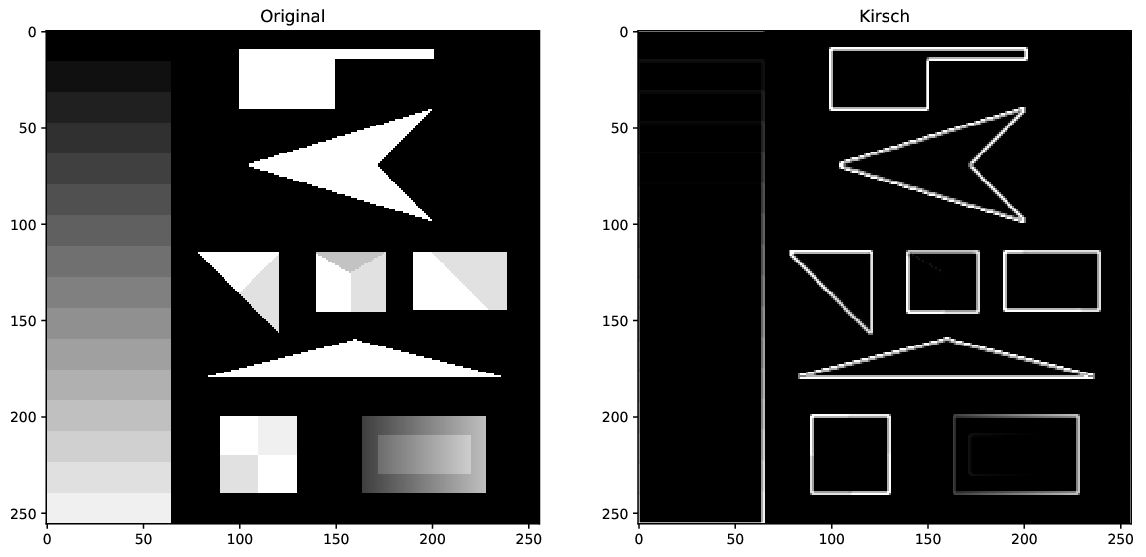
\includegraphics[height=6.5cm]{informe-imgs/ej3--test-original.jpg}
    \caption{\texttt{python3 practica6/ej3.py practica6/ej1-imgs/test-original.png }}
\end{figure}

\begin{figure}[H]
\centering
    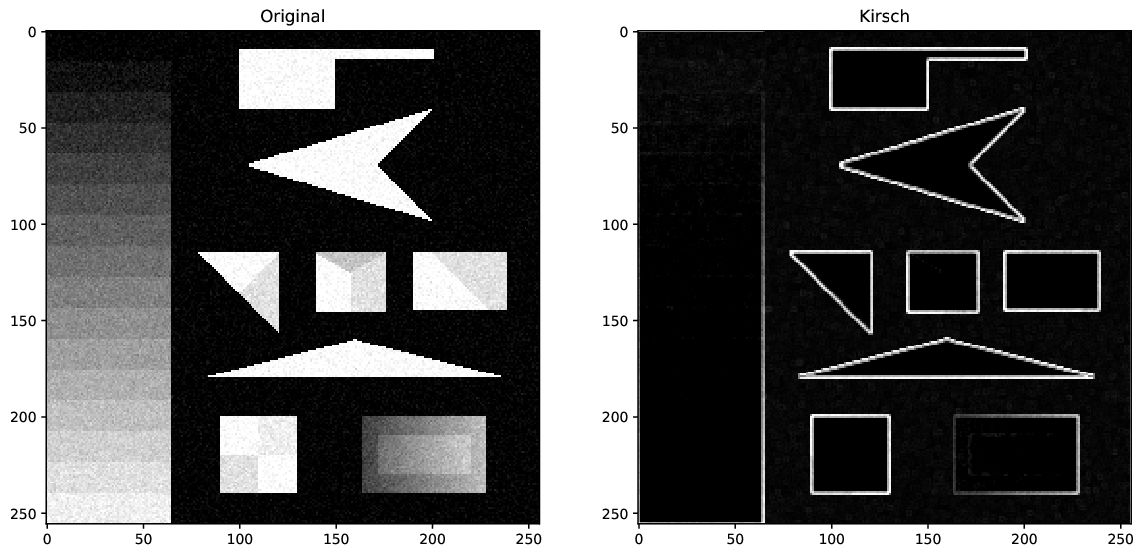
\includegraphics[height=6.5cm]{informe-imgs/ej3--test-gauss10.jpg}
    \caption{\texttt{python3 practica6/ej3.py practica6/ej1-imgs/test-gauss10.png }}
\end{figure}

\begin{figure}[H]
\centering
    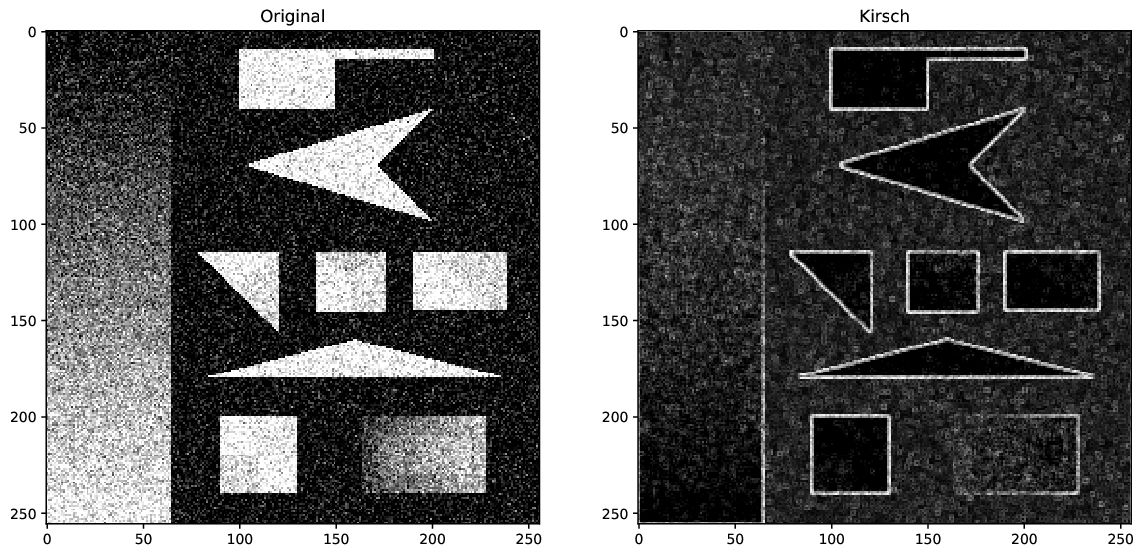
\includegraphics[height=6.5cm]{informe-imgs/ej3--test-gauss50.jpg}
    \caption{\texttt{python3 practica6/ej3.py practica6/ej1-imgs/test-gauss50.png }}
\end{figure}

\begin{figure}[H]
\centering
    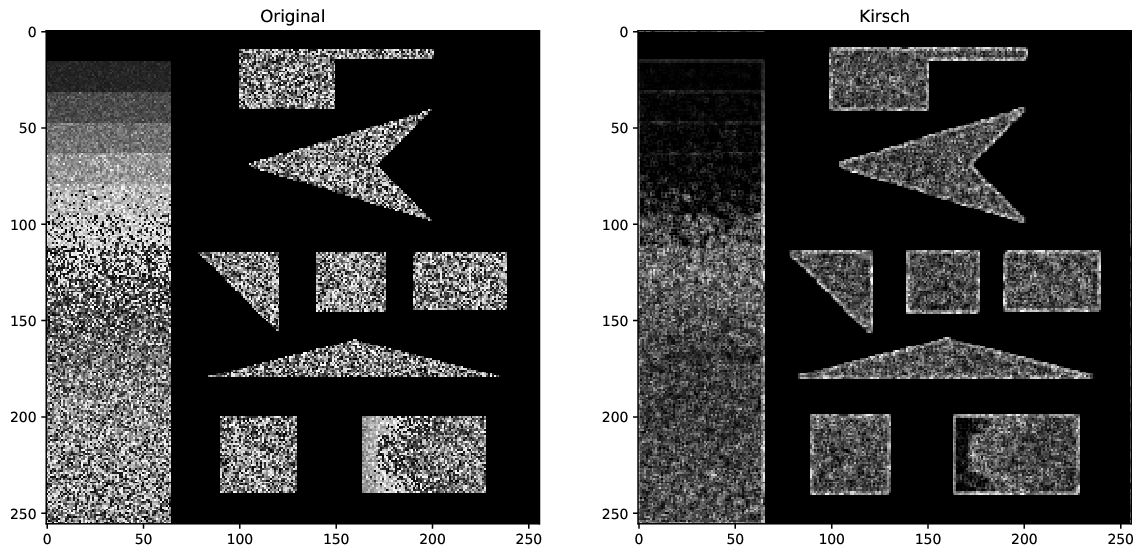
\includegraphics[height=6.5cm]{informe-imgs/ej3--test-rayleigh15.jpg}
    \caption{\texttt{python3 practica6/ej3.py practica6/ej1-imgs/test-rayleigh15.png }}
\end{figure}

\begin{figure}[H]
\centering
    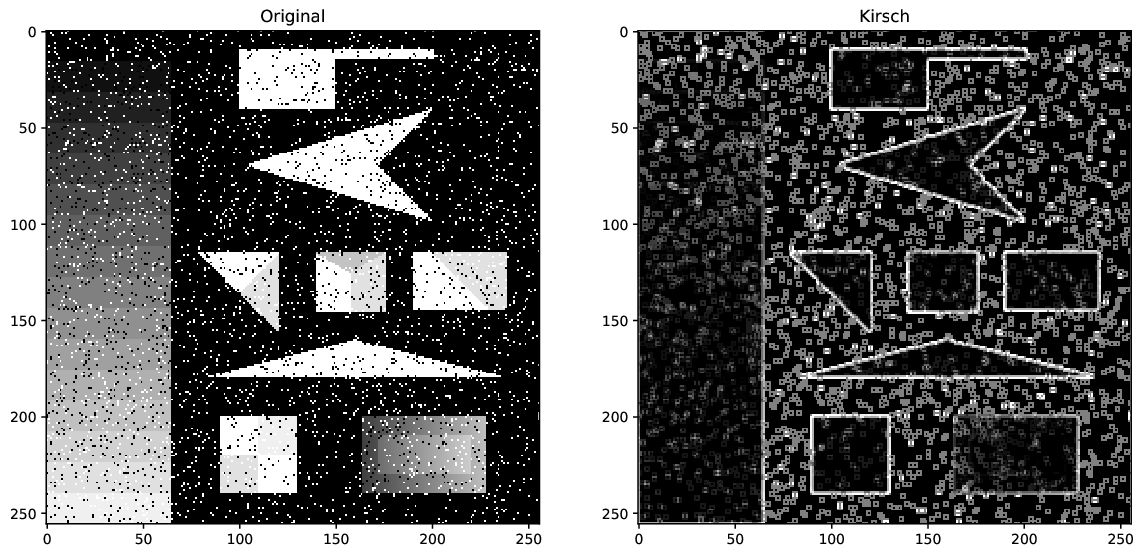
\includegraphics[height=6.5cm]{informe-imgs/ej3--test-saltpepper10.jpg}
    \caption{\texttt{python3 practica6/ej3.py practica6/ej1-imgs/test-saltpepper10.png }}
\end{figure}

\newpage
\section{Ejercicio 4: Algoritmo de Canny}

Modo de uso
\begin{verbatim}
    python3 practica6/ej4.py <img> <roberts|prewitt|sobel>
\end{verbatim}

El algoritmo de Canny se basa en los siguientes pasos.

\begin{enumerate}
\item Aplicarle un filtro gaussiano a la imagen. Esto lo que logra es suavizarla de manera que los filtros detectores de bordes funcionen mejor.
\item Aplicarle un filtro de detección de bordes, que devolverá para cada pixel un módulo y un ángulo del borde en ese pixel. En este caso probaremos con los filtros de detección de filtros de Roberts, Prewitt y Sobel. Explicaremos cada uno en su sección.
\item Dados el módulo y el ángulo del borde para cada pixel, haremos el paso de supresión de no-máximos. Este paso lo que hace es, para cada pixel, si en la dirección perpendicular a su borde hay otro pixel que tiene mayor módulo que él, entonces lo marcaremos como no-borde.
Esto lo que hace es que los bordes sean más finos, dado que para cada borde nos quedaremos solo con la tira de pixeles de mayor módulo.
\item Como el paso anterior puede afinar demasiado los bordes, puede desconectarlos. Por lo tanto, el último paso se llama umbral por histéresis y lo que hace es eso, chequear si en la dirección del borde hay pixeles con un cierto módulo de borde y en tal caso se marcarán como borde.
\end{enumerate}

Al final analizaremos los resultados.

Cada uno de los filtros que siguen se basan en convolucionar con dos siguientes matrices, una en la dirección $x$ y otra en $y$; y luego el resultado es el número complejo con coordenadas $(x,y)$. Lo que devolverá es el módulo y la fase de ese compeljo.



\subsection{Roberts}
Las matrices del filtro de Roberts son las siguientes.
\[
\mathbf{roberts_x} = \begin{bmatrix} 
1 & 0 \\
0 & -1
\end{bmatrix}
\]

\[
\mathbf{roberts_y} = \begin{bmatrix} 
0 & 1 \\
-1 & 0
\end{bmatrix}
\]

\begin{figure}[H]
\centering
    \includegraphics[height=6.5cm]{informe-imgs/ej4-roberts-lena-original.jpg}
    \caption{\texttt{python3 practica6/ej4.py practica6/ej1-imgs/lena-original.png roberts}}
\end{figure}

\begin{figure}[H]
\centering
    \includegraphics[height=6.5cm]{informe-imgs/ej4-roberts-lena-gauss10.jpg}
    \caption{\texttt{python3 practica6/ej4.py practica6/ej1-imgs/lena-gauss10.png roberts}}
\end{figure}

\begin{figure}[H]
\centering
    \includegraphics[height=6.5cm]{informe-imgs/ej4-roberts-lena-gauss50.jpg}
    \caption{\texttt{python3 practica6/ej4.py practica6/ej1-imgs/lena-gauss50.png roberts}}
\end{figure}

\begin{figure}[H]
\centering
    \includegraphics[height=6.5cm]{informe-imgs/ej4-roberts-lena-rayleigh15.jpg}
    \caption{\texttt{python3 practica6/ej4.py practica6/ej1-imgs/lena-rayleigh15.png roberts}}
\end{figure}

\begin{figure}[H]
\centering
    \includegraphics[height=6.5cm]{informe-imgs/ej4-roberts-lena-saltpepper10.jpg}
    \caption{\texttt{python3 practica6/ej4.py practica6/ej1-imgs/lena-saltpepper10.png roberts}}
\end{figure}


\begin{figure}[H]
\centering
    \includegraphics[height=6.5cm]{informe-imgs/ej4-roberts-test-original.jpg}
    \caption{\texttt{python3 practica6/ej4.py practica6/ej1-imgs/test-original.png roberts}}
\end{figure}

\begin{figure}[H]
\centering
    \includegraphics[height=6.5cm]{informe-imgs/ej4-roberts-test-gauss10.jpg}
    \caption{\texttt{python3 practica6/ej4.py practica6/ej1-imgs/test-gauss10.png roberts}}
\end{figure}

\begin{figure}[H]
\centering
    \includegraphics[height=6.5cm]{informe-imgs/ej4-roberts-test-gauss50.jpg}
    \caption{\texttt{python3 practica6/ej4.py practica6/ej1-imgs/test-gauss50.png roberts}}
\end{figure}

\begin{figure}[H]
\centering
    \includegraphics[height=6.5cm]{informe-imgs/ej4-roberts-test-rayleigh15.jpg}
    \caption{\texttt{python3 practica6/ej4.py practica6/ej1-imgs/test-rayleigh15.png roberts}}
\end{figure}

\begin{figure}[H]
\centering
    \includegraphics[height=6.5cm]{informe-imgs/ej4-roberts-test-saltpepper10.jpg}
    \caption{\texttt{python3 practica6/ej4.py practica6/ej1-imgs/test-saltpepper10.png roberts}}
\end{figure}


\newpage
\subsection{Prewitt}
Las matrices del filtro de Prewitt son las siguientes.
\[
\mathbf{prewitt_x} = \begin{bmatrix} 
-1 & 0 & 1 \\
-1 & 0 & 1 \\
-1 & 0 & 1 \\
\end{bmatrix}
\]

\[
\mathbf{prewitt_y} = \begin{bmatrix} 
1 & 1 & 1 \\
0 & 0 & 0 \\
-1 & -1 & -1 \\
\end{bmatrix}
\]

\begin{figure}[H]
\centering
    \includegraphics[height=6.5cm]{informe-imgs/ej4-prewitt-lena-original.jpg}
    \caption{\texttt{python3 practica6/ej4.py practica6/ej1-imgs/lena-original.png prewitt}}
\end{figure}

\begin{figure}[H]
\centering
    \includegraphics[height=6.5cm]{informe-imgs/ej4-prewitt-lena-gauss10.jpg}
    \caption{\texttt{python3 practica6/ej4.py practica6/ej1-imgs/lena-gauss10.png prewitt}}
\end{figure}

\begin{figure}[H]
\centering
    \includegraphics[height=6.5cm]{informe-imgs/ej4-prewitt-lena-gauss50.jpg}
    \caption{\texttt{python3 practica6/ej4.py practica6/ej1-imgs/lena-gauss50.png prewitt}}
\end{figure}

\begin{figure}[H]
\centering
    \includegraphics[height=6.5cm]{informe-imgs/ej4-prewitt-lena-rayleigh15.jpg}
    \caption{\texttt{python3 practica6/ej4.py practica6/ej1-imgs/lena-rayleigh15.png prewitt}}
\end{figure}

\begin{figure}[H]
\centering
    \includegraphics[height=6.5cm]{informe-imgs/ej4-prewitt-lena-saltpepper10.jpg}
    \caption{\texttt{python3 practica6/ej4.py practica6/ej1-imgs/lena-saltpepper10.png prewitt}}
\end{figure}


\begin{figure}[H]
\centering
    \includegraphics[height=6.5cm]{informe-imgs/ej4-prewitt-test-original.jpg}
    \caption{\texttt{python3 practica6/ej4.py practica6/ej1-imgs/test-original.png prewitt}}
\end{figure}

\begin{figure}[H]
\centering
    \includegraphics[height=6.5cm]{informe-imgs/ej4-prewitt-test-gauss10.jpg}
    \caption{\texttt{python3 practica6/ej4.py practica6/ej1-imgs/test-gauss10.png prewitt}}
\end{figure}

\begin{figure}[H]
\centering
    \includegraphics[height=6.5cm]{informe-imgs/ej4-prewitt-test-gauss50.jpg}
    \caption{\texttt{python3 practica6/ej4.py practica6/ej1-imgs/test-gauss50.png prewitt}}
\end{figure}

\begin{figure}[H]
\centering
    \includegraphics[height=6.5cm]{informe-imgs/ej4-prewitt-test-rayleigh15.jpg}
    \caption{\texttt{python3 practica6/ej4.py practica6/ej1-imgs/test-rayleigh15.png prewitt}}
\end{figure}

\begin{figure}[H]
\centering
    \includegraphics[height=6.5cm]{informe-imgs/ej4-prewitt-test-saltpepper10.jpg}
    \caption{\texttt{python3 practica6/ej4.py practica6/ej1-imgs/test-saltpepper10.png prewitt}}
\end{figure}



\newpage
\subsection{Sobel}
Las matrices del filtro de Sobel son las siguientes.
\[
\mathbf{sobel_x} = \begin{bmatrix} 
1 & 0 & -1 \\
2 & 0 & -2 \\
1 & 0 & -1 \\
\end{bmatrix}
\]

\[
\mathbf{sobel_y} = \begin{bmatrix} 
1 & 1 & 1 \\
0 & 0 & 0 \\
-1 & -2 & -1 \\
\end{bmatrix}
\]

\begin{figure}[H]
\centering
    \includegraphics[height=6.5cm]{informe-imgs/ej4-sobel-lena-original.jpg}
    \caption{\texttt{python3 practica6/ej4.py practica6/ej1-imgs/lena-original.png sobel}}
\end{figure}

\begin{figure}[H]
\centering
    \includegraphics[height=6.5cm]{informe-imgs/ej4-sobel-lena-gauss10.jpg}
    \caption{\texttt{python3 practica6/ej4.py practica6/ej1-imgs/lena-gauss10.png sobel}}
\end{figure}

\begin{figure}[H]
\centering
    \includegraphics[height=6.5cm]{informe-imgs/ej4-sobel-lena-gauss50.jpg}
    \caption{\texttt{python3 practica6/ej4.py practica6/ej1-imgs/lena-gauss50.png sobel}}
\end{figure}

\begin{figure}[H]
\centering
    \includegraphics[height=6.5cm]{informe-imgs/ej4-sobel-lena-rayleigh15.jpg}
    \caption{\texttt{python3 practica6/ej4.py practica6/ej1-imgs/lena-rayleigh15.png sobel}}
\end{figure}

\begin{figure}[H]
\centering
    \includegraphics[height=6.5cm]{informe-imgs/ej4-sobel-lena-saltpepper10.jpg}
    \caption{\texttt{python3 practica6/ej4.py practica6/ej1-imgs/lena-saltpepper10.png sobel}}
\end{figure}


\begin{figure}[H]
\centering
    \includegraphics[height=6.5cm]{informe-imgs/ej4-sobel-test-original.jpg}
    \caption{\texttt{python3 practica6/ej4.py practica6/ej1-imgs/test-original.png sobel}}
\end{figure}

\begin{figure}[H]
\centering
    \includegraphics[height=6.5cm]{informe-imgs/ej4-sobel-test-gauss10.jpg}
    \caption{\texttt{python3 practica6/ej4.py practica6/ej1-imgs/test-gauss10.png sobel}}
\end{figure}

\begin{figure}[H]
\centering
    \includegraphics[height=6.5cm]{informe-imgs/ej4-sobel-test-gauss50.jpg}
    \caption{\texttt{python3 practica6/ej4.py practica6/ej1-imgs/test-gauss50.png sobel}}
\end{figure}

\begin{figure}[H]
\centering
    \includegraphics[height=6.5cm]{informe-imgs/ej4-sobel-test-rayleigh15.jpg}
    \caption{\texttt{python3 practica6/ej4.py practica6/ej1-imgs/test-rayleigh15.png sobel}}
\end{figure}

\begin{figure}[H]
\centering
    \includegraphics[height=6.5cm]{informe-imgs/ej4-sobel-test-saltpepper10.jpg}
    \caption{\texttt{python3 practica6/ej4.py practica6/ej1-imgs/test-saltpepper10.png sobel}}
\end{figure}

\newpage
\subsection{Conclusión}

Como puede observarse, todos los filtros andan muy bien para las imágenes sin ruido. Detectan los bordes a la perfección en esos casos, y los filtros que dan son muy adecuados: son angostos pero no están quebrados.

Además, para el caso de ruido gaussiano con media 10 también son resilientes y andan muy bien, casi seguramente debido al filtro gaussiano que se le pasa antes de empezar el algoritmo, y el umbral por histéresis, que une bordes que el ruido puede haber eliminado.

Sin embargo, ya en las imágenes con ruido los filtros se comportan de manera muy errática.
En la imagen contaminada con ruido sal y pimienta, un humano puede detectar los bordes casi a la perfección, pero nuestro algoritmo falla completamente, lo cual es un punto claramente débil.


\end{document}
